\documentclass[a4paper]{article}
\usepackage{float}
\usepackage[margin=1.2in]{geometry}
\usepackage[english]{babel}
\usepackage[utf8]{inputenc}
\usepackage{amsmath}
\usepackage{subcaption}
\usepackage{graphicx}
\usepackage{hyperref}
\usepackage{listings}
\usepackage[colorinlistoftodos]{todonotes}
\title{Student Discourse Through the Years}

\author{Benji Lu, Kai Fukutaki, Ziqi Xiong}

\date{\today}

\usepackage{Sweave}
\begin{document}
\maketitle

\Sconcordance{concordance:FinalProject.tex:FinalProject.Rnw:%
1 17 1 1 0 4 1 1 9 32 1 1 2 1 0 2 1 11 0 1 2 4 1 1 2 1 0 1 2 1 0 2 1 10 %
0 1 2 12 0 1 2 4 1 1 8 7 0 2 1 8 0 1 1 11 0 1 2 2 1 1 2 5 0 1 2 3 1 1 2 %
1 0 1 1 17 0 1 2 9 1 1 2 5 0 1 2 6 1 1 2 5 0 1 2 6 1 1 2 5 0 1 2 4 1 1 %
2 1 0 1 1 8 0 1 2 4 1 1 2 1 0 1 1 8 0 1 2 4 1 1 2 1 0 1 1 8 0 1 2 4 1 1 %
4 2 1 1 22 1 8 11 0 1 2 4 1 1 10 13 0 1 2 4 1 1 6 1 5 8 0 1 2 2 1 1 2 1 %
0 1 9 8 0 1 2 5 0 1 2 4 1 1 12 25 0 1 2 1 7 4 1 1 8 17 0 1 2 4 1 1 9 17 %
0 1 2 2 1 1 6 9 0 1 2 5 1 1 10 13 0 1 2 21 1}




\section{Motivation}
They say that those who do not know history are doomed to repeat it. We hope to show how campus dialogue on the Claremont Colleges has changed over time, using articles from The Student Life as representative of the discourse surrounding hot-button issues on campus. The Student Life, or TSL, is the oldest college newspaper in Southern California, and it is student-written and managed. It thus serves as a good glimpse into the thoughts and discourse of the students of the 5 Claremont Colleges (Pomona, Claremont McKenna, Scripps, Pitzer, Harvey Mudd). The student population itself is in a constant state of flux, as students generally spend only 4-5 years on campus. This ever changing population, and thus ever changing set of TSL writers (especially given that writers are probably working for TSL during their whole time on campus), means that issues in campus dialogue can repeatedly resurface when current students are not aware of the college discussions that took place four or five years ago. Plus, TSL does not have a `` static''  format; the number of articles published in each issue depends on the number of articles written, rather than publishing the same length paper each week. This allows for interesting data on word usage trends, topics covered, authorship, and more over time. How are topics evolving over time? Can we see major spikes in certain topics/phrases and trace those back to major events? Can we use these trends to inform our current dialogue? With better, more easily accessible information on TSL history, we can make it easier for future students to see what kind of discussion and action has taken place at the Claremont Colleges so that they can better understand the history of intellectual conversations on our campus and create fresher, deeper discussions in the future.

\section{Methodology}

\subsection{Data Source}

Our raw data was acquired directly from TSL's SQL database on ASPC peninsula server. The data is in the format of three csv tables: 

\begin{enumerate}
\item \textbf{articles}: This table contains the information related to the TSL articles, including id, title, content, status (published or not), created date, published date, updated date, section id and issue id.
\item \textbf{profiles}: This table contains the information related to the TSL staff, including id, name and position.
\item \textbf{articles\_profiles}: This table contains the authorship of TSL articles. Each row contains a TSL staff member id and an article id.
\end{enumerate}

We joined the three tables by article\_id and profile\_id and filtered out all the articles that are not published, do not have enough content (body text less than 50 words), or miss author or published date information. We selected important variables including title, content, published date, and author's name for our analysis.

To access the data we used, visit our code repository at \href{https://github.com/ZiqiXiong/TopicModeling}{https://github.com/ZiqiXiong/TopicModeling}.

\subsection{Model Training}

Our goal is to build an unsupervised model that cluster the TSL articles by their similarity in word usage so that each cluster can be labeled later and studied as a topic. With that goal in mind, we studied and used Latent Dirichlet Allocation(LDA) developed by Andrew Ng, et al., in 2003 for our project. LDA is a probabilistic model that allows sets of observations to be explained by unobserved groups that explain why some parts of the data are similar. When applied to a collection of text documents, LDA views each document as a mixture of a small number of topics and each word generated by one of the document's topics. With different inference techniques such as Gibbs Sampling, LDA is able to learn the composition of each topic (its associated word probabilities) and the topic mixture of each document.

Before training our LDA model, we first processed the body text of TSL articles by converting all words to lower case and reducing words to their stems, so that a group of words such as `` study'' ,`` Study''  and `` studies''  can be treated as one. We also removed punctuation, stop words (the most common, short function words), and extremely rare words that would only add noise to our model training. Finally, we transformed the collection of articles into a document-term matrix with each row representing an article and column representing a word. 

By using the R package `` topicmodel'', We trained multiple LDA models with different numbers of topics as input, including 25, 30, 35, 40, 45 and 50, so that we can use the most suitable model in our analysis later depending on how general we want the topics to be.

\subsection{Result and Visualization}

Our LDA model is capable of clustering key words into human-recognizable topic. Take five random topics discovered by our 40-topic model as an example:

\begin{Schunk}
\begin{Sinput}
> topic.terms = get.topic.terms(topic.model,20)
> set.seed(47)
> topic.terms[1:5,sample(40,5)]
\end{Sinput}
\begin{Soutput}
     Topic 40  Topic 15  Topic 29    Topic 31   Topic 21
[1,] "music"   "sex"     "student"   "student"  "game"  
[2,] "perform" "partner" "event"     "protest"  "fan"   
[3,] "song"    "feel"    "claremont" "black"    "player"
[4,] "band"    "sexual"  "communiti" "support"  "play"  
[5,] "play"    "make"    "colleg"    "movement" "season"
\end{Soutput}
\end{Schunk}

The 5 topics can be easily identified as ``music'', ``sex'', ``campus event'', ``student protest'', and ``sports game'' by their top keywords.

In addition to the distribution of words in topics, the LDA model can also calculates the percentage of a topic in an article and infers what the article is about. Take five random TSL articles for example:

\begin{Schunk}
\begin{Sinput}
> set.seed(37)
> # The primary topic of five articles
> sample.articles = articles[sample(5000,5),c(2,8)]
> names(sample.articles) = c('article.title','primary.topic')
> sample.articles
\end{Sinput}
\begin{Soutput}
                                              article.title primary.topic
2749 Women's Basketball Struggles Through Tough First Games             1
395       Peace, Popular Opinion, and the Prisoner Exchange            16
3243        Panel at CMC Debates Approach to Syria Conflict            10
2483                  Students Put Out Fire in Scripps Dorm            34
3592 Ye Olde TSL: 1927, The First Year of the Sponsor Group            27
\end{Soutput}
\begin{Sinput}
> # What the topics are about
> topic.terms[1:5, sample.articles[['primary.topic']]]
\end{Sinput}
\begin{Soutput}
     Topic 1   Topic 16 Topic 10  Topic 34  Topic 27 
[1,] "game"    "polit"  "student" "campus"  "student"
[2,] "sagehen" "state"  "discuss" "hall"    "pomona" 
[3,] "score"   "govern" "issu"    "student" "program"
[4,] "team"    "obama"  "chang"   "build"   "sponsor"
[5,] "sciac"   "presid" "talk"    "resid"   "colleg" 
\end{Soutput}
\end{Schunk}

As we can see from the result above, ``Women's Basketball Struggles Through Tough First Games'' is categorized into topic 1 about team sports, ``Peace, Popular Opinion, and the Prisoner Exchange'' into topic 16 about national politics, ``Panel at CMC Debates Approach to Syria Conflict'' into topic 10 about student discussion, `` Students Put Out Fire in Scripps Dorm'' into topic 34 about residential life, and ``Ye Olde TSL: 1927, The First Year of the Sponsor Group'' into topic 27 about Pomona sponsor program. 

Our model can also discover topics in articles that are not in our TSL dataset. For example, it can successfully categorize an 108-word excerpt from Martin Luther King's speech ``I Have a Dream'' into topic 16 about national politics and topic 31 about student protest.

\begin{Schunk}
\begin{Sinput}
> test.paragraph = "I have a dream that one day on the red hills of Georgia, 
+ the sons of former slaves and the sons of former slave owners will be able to sit down 
+ together at the table of brotherhood. I have a dream that one day even the state 
+ of Mississippi, a state sweltering with the heat of injustice, sweltering with the heat 
+ of oppression, will be transformed into an oasis of freedom and justice. I have a dream that 
+ my four little children will one day live in a nation where they will not be judged by the 
+ color of their skin but by the content of their character."
> test.result = classifyResult(test.paragraph,topic.model)
> test.result
\end{Sinput}
\begin{Soutput}
   Topic.ID    Weight
16       16 0.2469187
31       31 0.1954415
3         3 0.1920453
\end{Soutput}
\begin{Sinput}
> topic.terms[1:5, test.result[['Topic.ID']]]
\end{Sinput}
\begin{Soutput}
     Topic 16 Topic 31   Topic 3  
[1,] "polit"  "student"  "film"   
[2,] "state"  "protest"  "show"   
[3,] "govern" "black"    "charact"
[4,] "obama"  "support"  "movi"   
[5,] "presid" "movement" "play"   
\end{Soutput}
\end{Schunk}

After categorizing each article into its related topics, we are able to plot the frequency of a topic over time by counting the number of its articles every week. For example, here is the plot of topic 31 about student protest:

\begin{Schunk}
\begin{Sinput}
> topicgraph(articles,31,2,14)
\end{Sinput}
\end{Schunk}
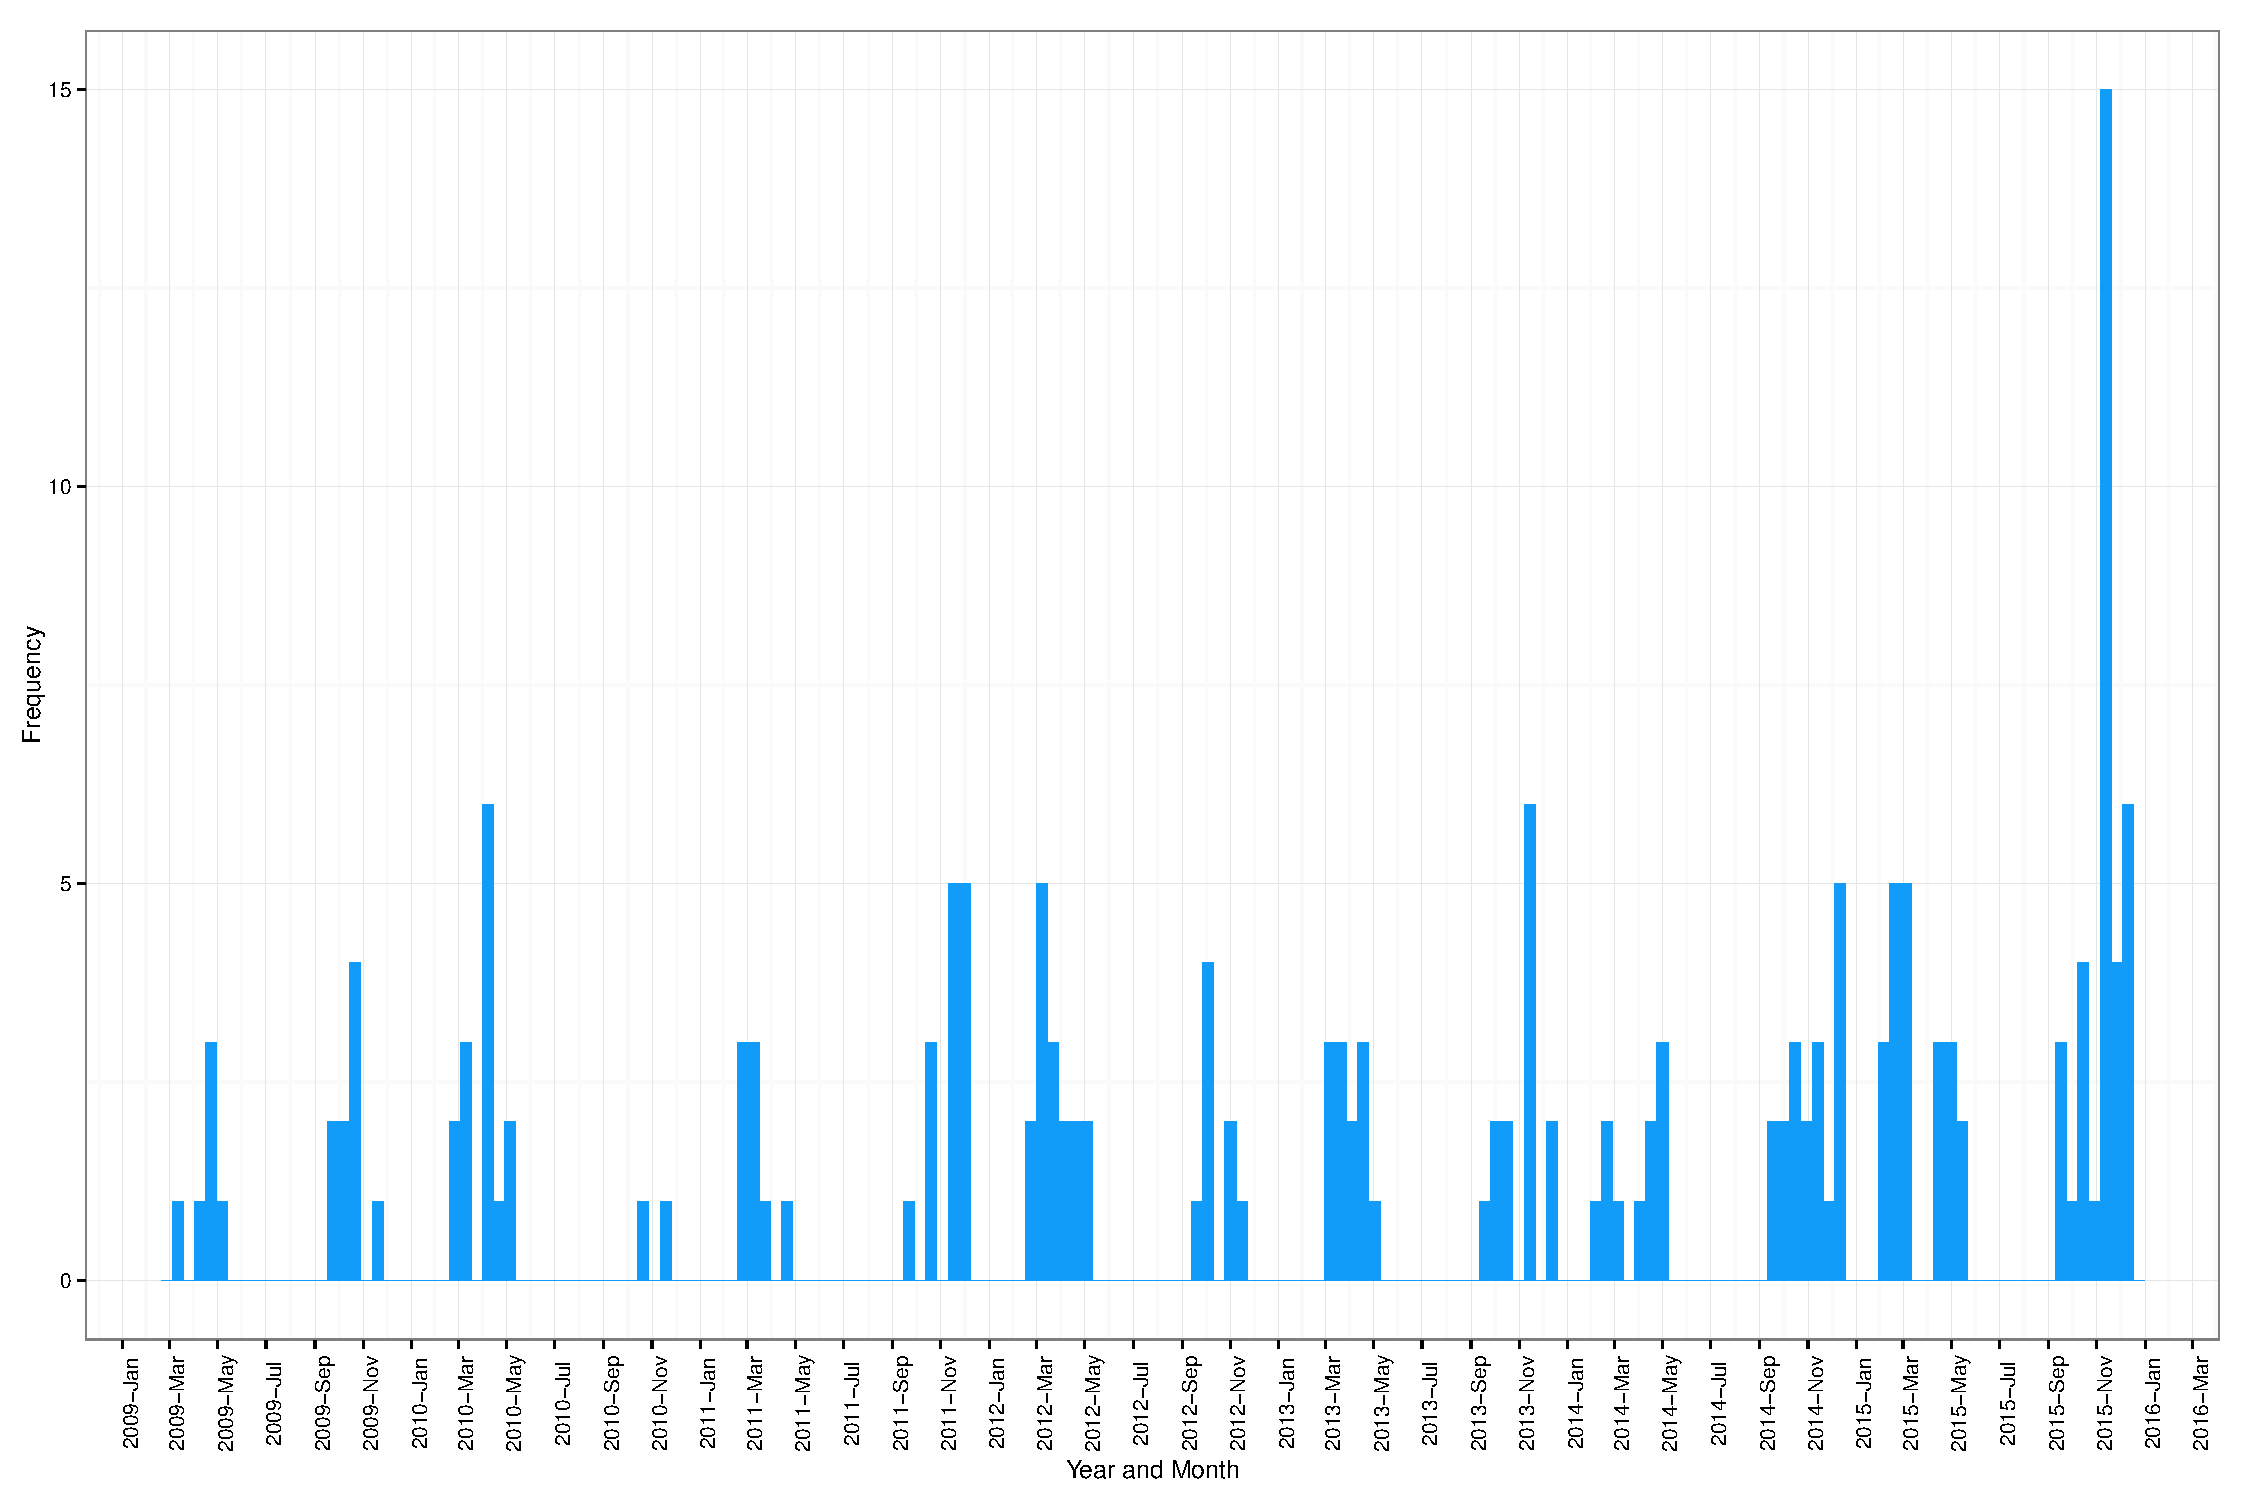
\includegraphics{FinalProject-005}

As we can see from the plot, the frequency of topic 31 experienced an unprecedented spike during the 2015 Fall semester, which reflects the heated discussion on the series of college protests in Yale, Mizzou and Claremont McKenna this fall.

We can also visualize what topics each author writes about. Take TSL editorial board for example: 

\begin{Schunk}
\begin{Sinput}
> print(authorChart2(articles,'Editorial Board',2))
> topic.terms[1:10,c(10,19)]
\end{Sinput}
\begin{Soutput}
      Topic 10   Topic 19 
 [1,] "student"  "write"  
 [2,] "discuss"  "book"   
 [3,] "issu"     "read"   
 [4,] "chang"    "stori"  
 [5,] "talk"     "articl" 
 [6,] "question" "tsl"    
 [7,] "campus"   "news"   
 [8,] "import"   "writer" 
 [9,] "pomona"   "media"  
[10,] "colleg"   "publish"
\end{Soutput}
\end{Schunk}
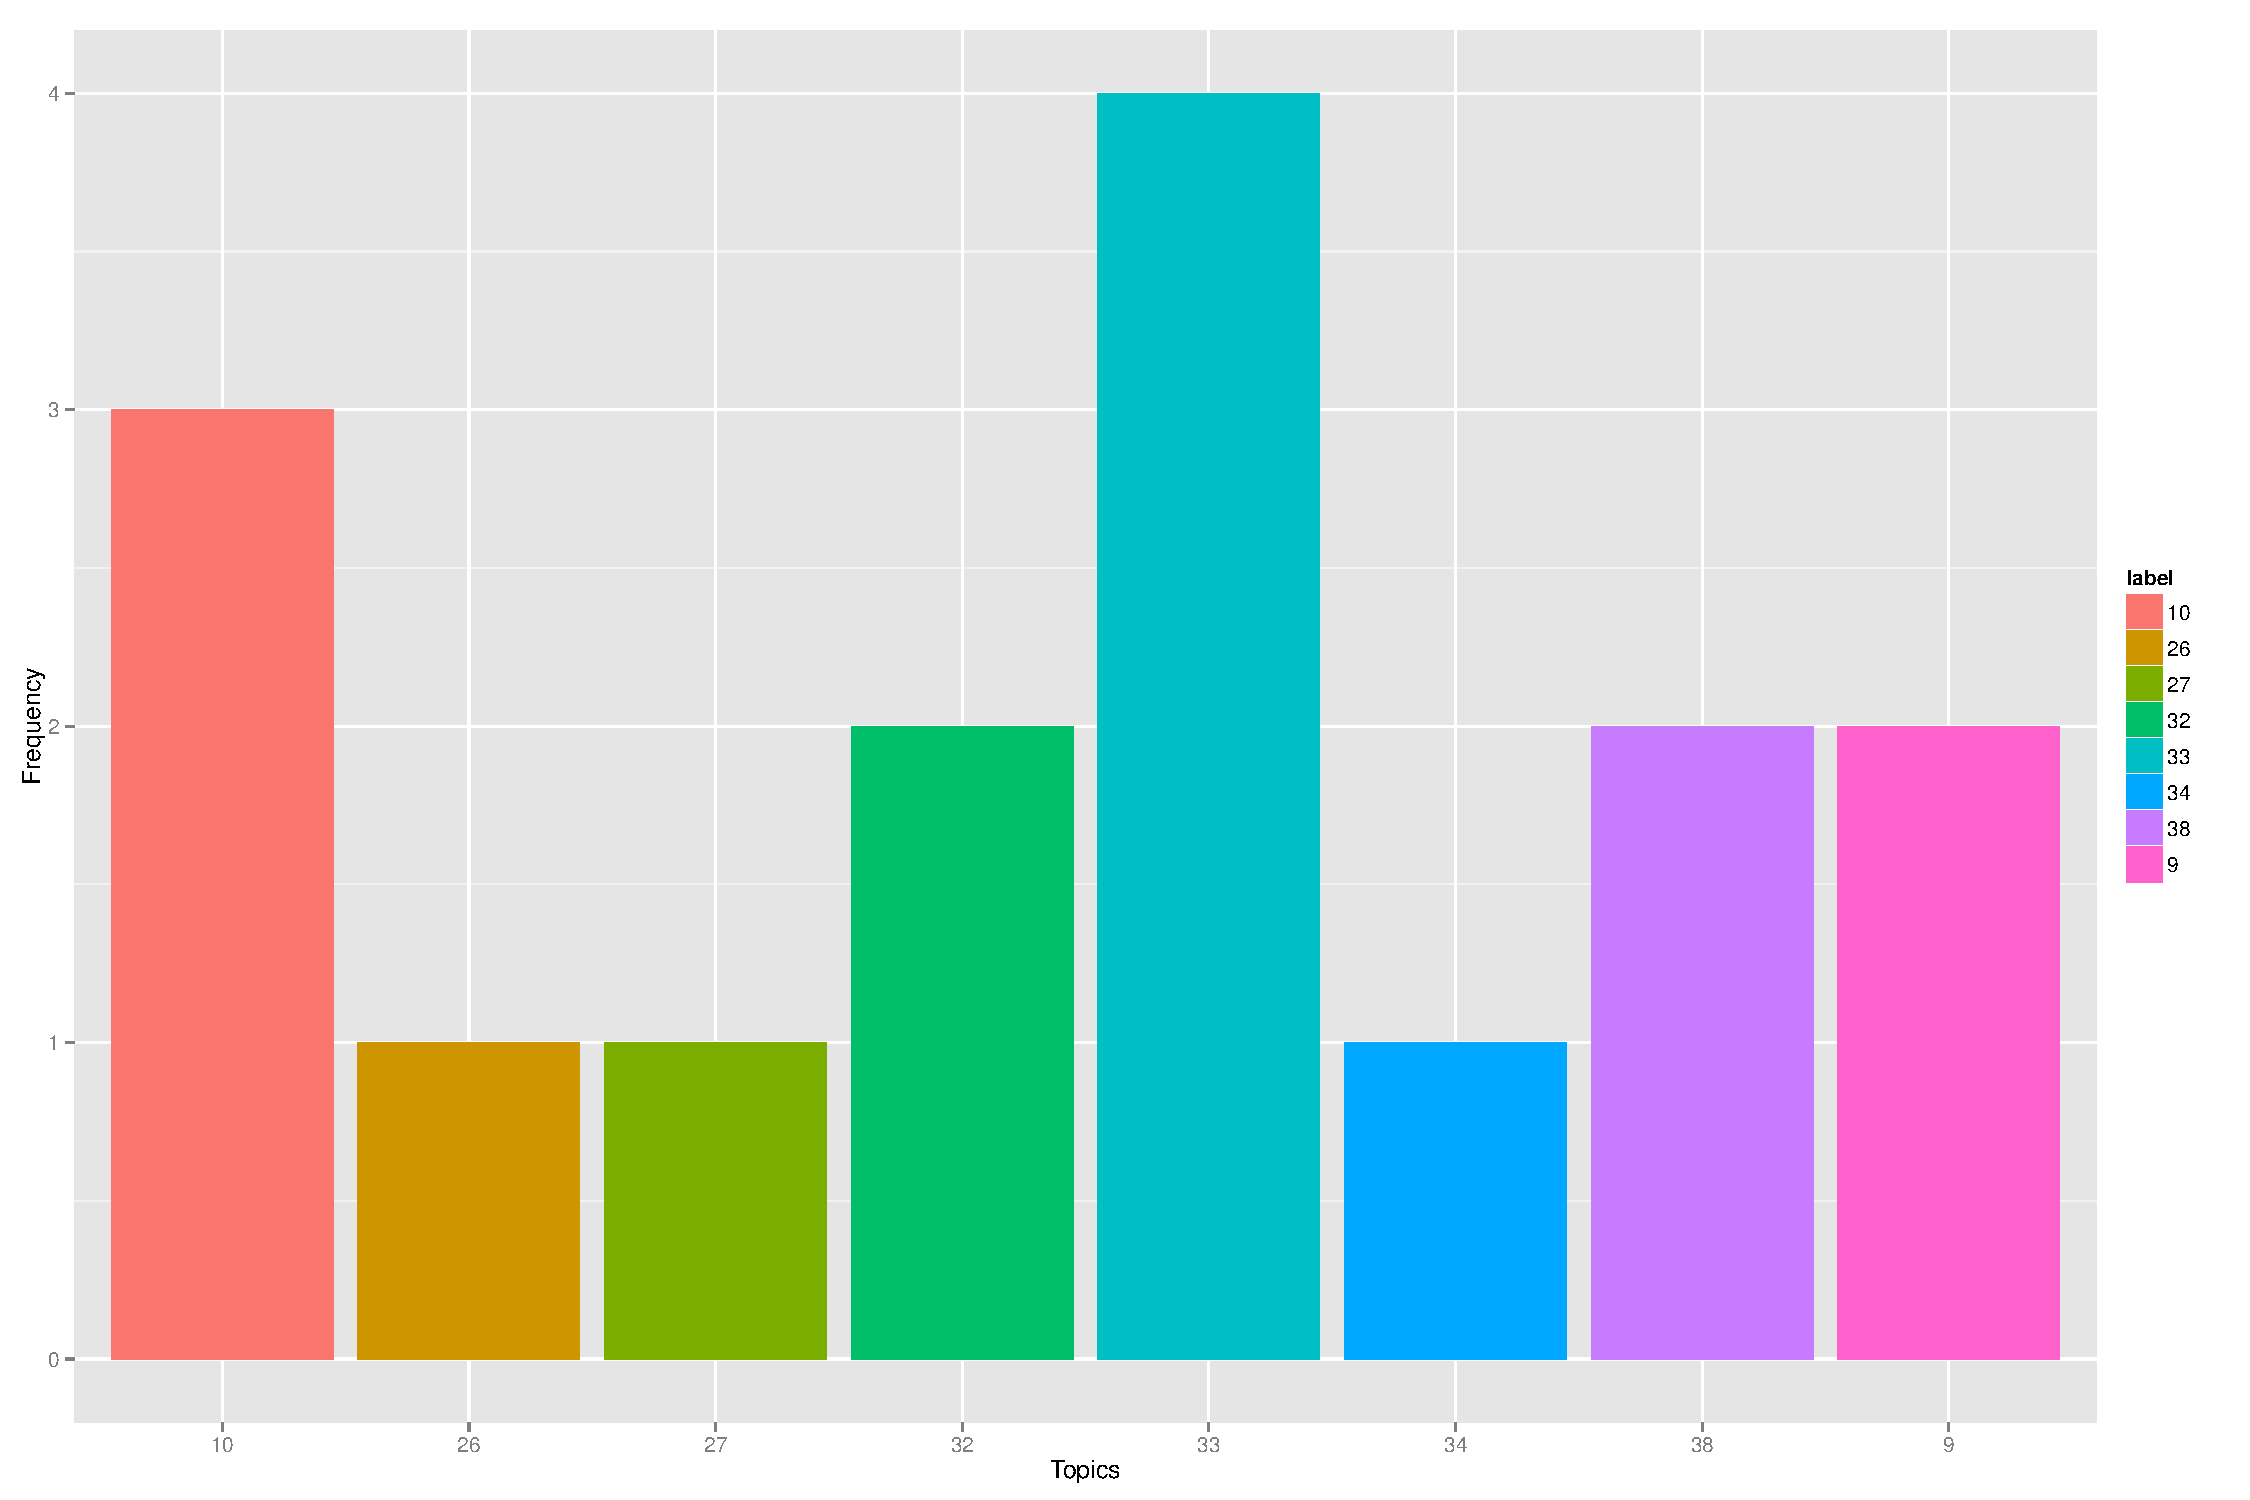
\includegraphics{FinalProject-006}

The plot shows that TSL editorial board writes most about topic 10 about student discussions and topic 19 about campus media, which are indeed what editors typically voice their opinions about. 

\section{Findings}

\subsection{Topic Analysis}

Here, we highlight some interesting findings that we discovered through our topic analysis, beginning with topic trends.

Two prominent movements in the recent history of the Claremont Colleges are the divestment campaign and the push for the unionization of the Pomona's dining hall workers. Using our model's visualizations of topics over time, we found the following trend of \textit{TSL}'s coverage of the two topics:

\begin{Schunk}
\begin{Sinput}
> topicgraph(articles,11,2,14)
\end{Sinput}
\end{Schunk}
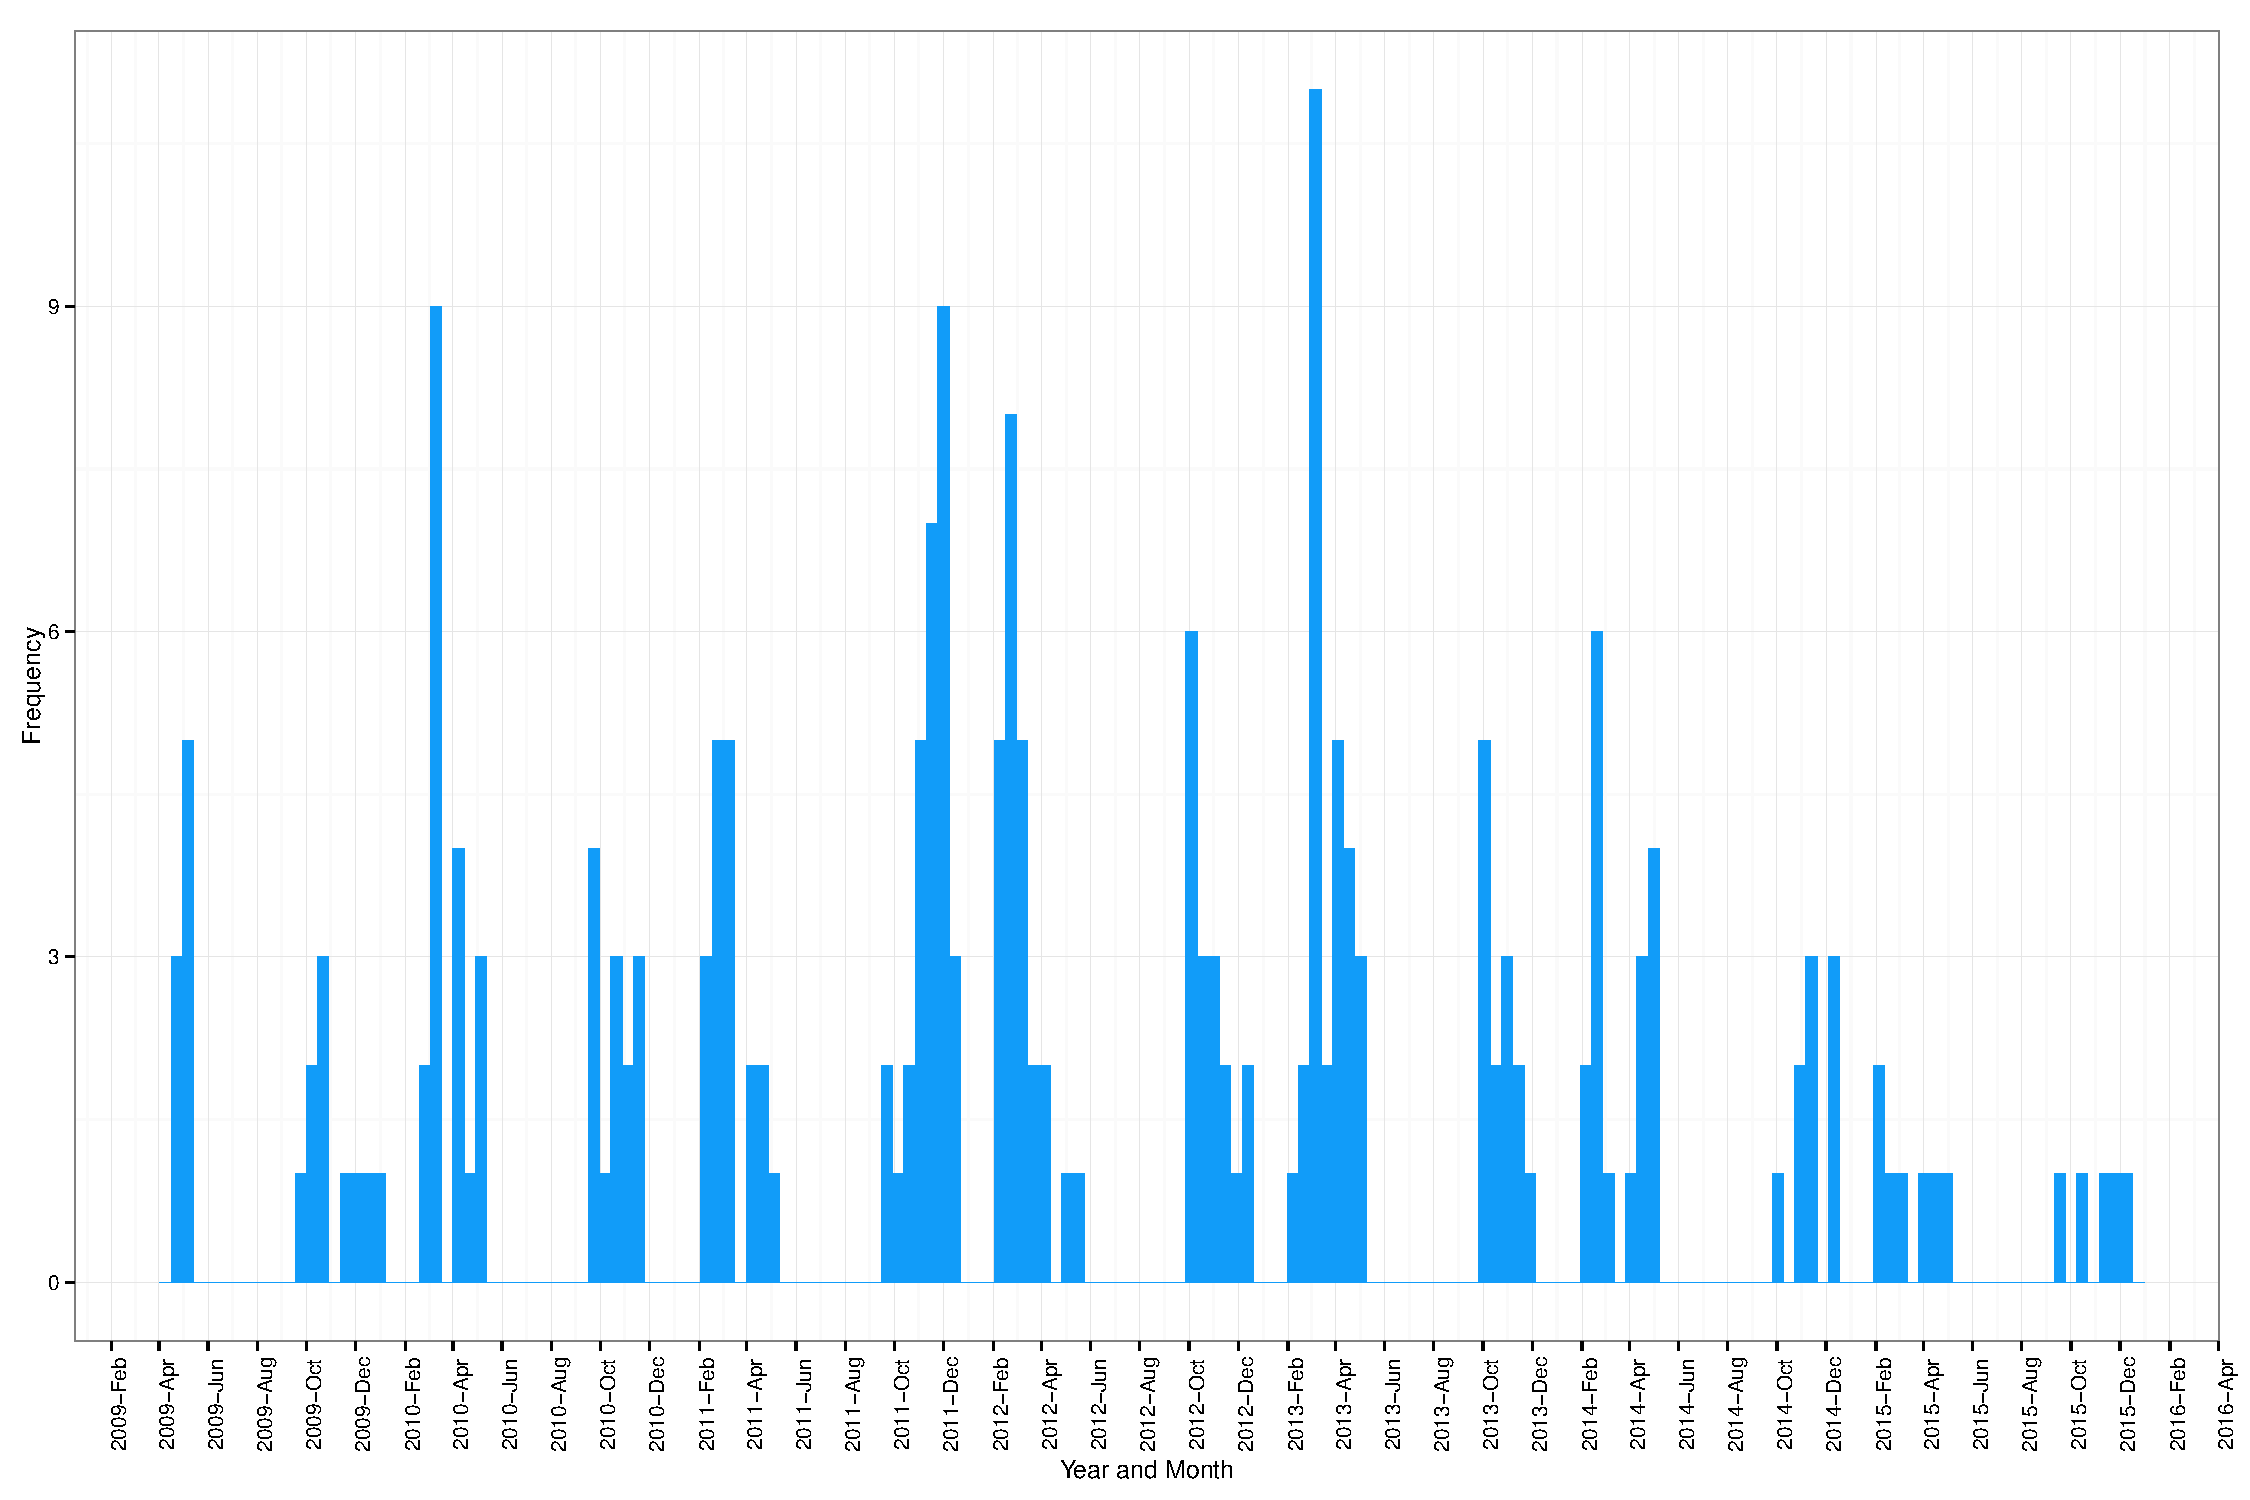
\includegraphics{FinalProject-007}

The graph shows that \textit{TSL} coverage of the two topics was robust from the spring of 2009 up to and including the spring of 2013. In particular, it reached its height between the fall of 2011 and the spring of 2013. Some interesting article headlines include ``NLRB Will Investigate Labor Practice Charges at Pomona Dining Halls'' at the peak in December 2011, ``WFJ Votes to Unionize'' at the very end of May 2013, ``Pomona Opts Not to Divest'' in October 2013, and``Pitzer College to Divest From Fossil Fuel Funds'' around April of 2014.

Unfortunately, our model wasn't able to separate the two topics, but the results are nonetheless fascinating. From our own perspective as juniors at Pomona College, the visualization is especially illuminating. We came to Pomona in the fall of 2013, right at the tail end of the peaks of the dining hall and divestment movements, as the visualization accurately shows. The semester before we arrived, the dining hall workers voted to unionize; the semester we arrived, President David Oxtoby announced Pomona's decision not to divest from fossil fuels; and the semester after we arrived, Pitzer College announced that it would divest from fossil fuels. Shortly after that, the discussions about the two topics died down, both in \textit{TSL} and in general campus discourse. Regardless of one's opinions on these issues, they were exciting events in the colleges' history, and while we were able to witness the ultimate outcomes, we had virutally no knowledge of the related events and discussions that preceded the outcomes. With the visualizations our model provides, we're now better able to access key institutional memory in the form of \textit{TSL} coverage of the topics in order to understand these outcomes in their broader context that spans several years.

Another interesting topic that has been trending recently in \textit{TSL} coverage is sexual assault. Here's the graph that our model produced:

\begin{Schunk}
\begin{Sinput}
> topicgraph(articles,20,2,14)
\end{Sinput}
\end{Schunk}
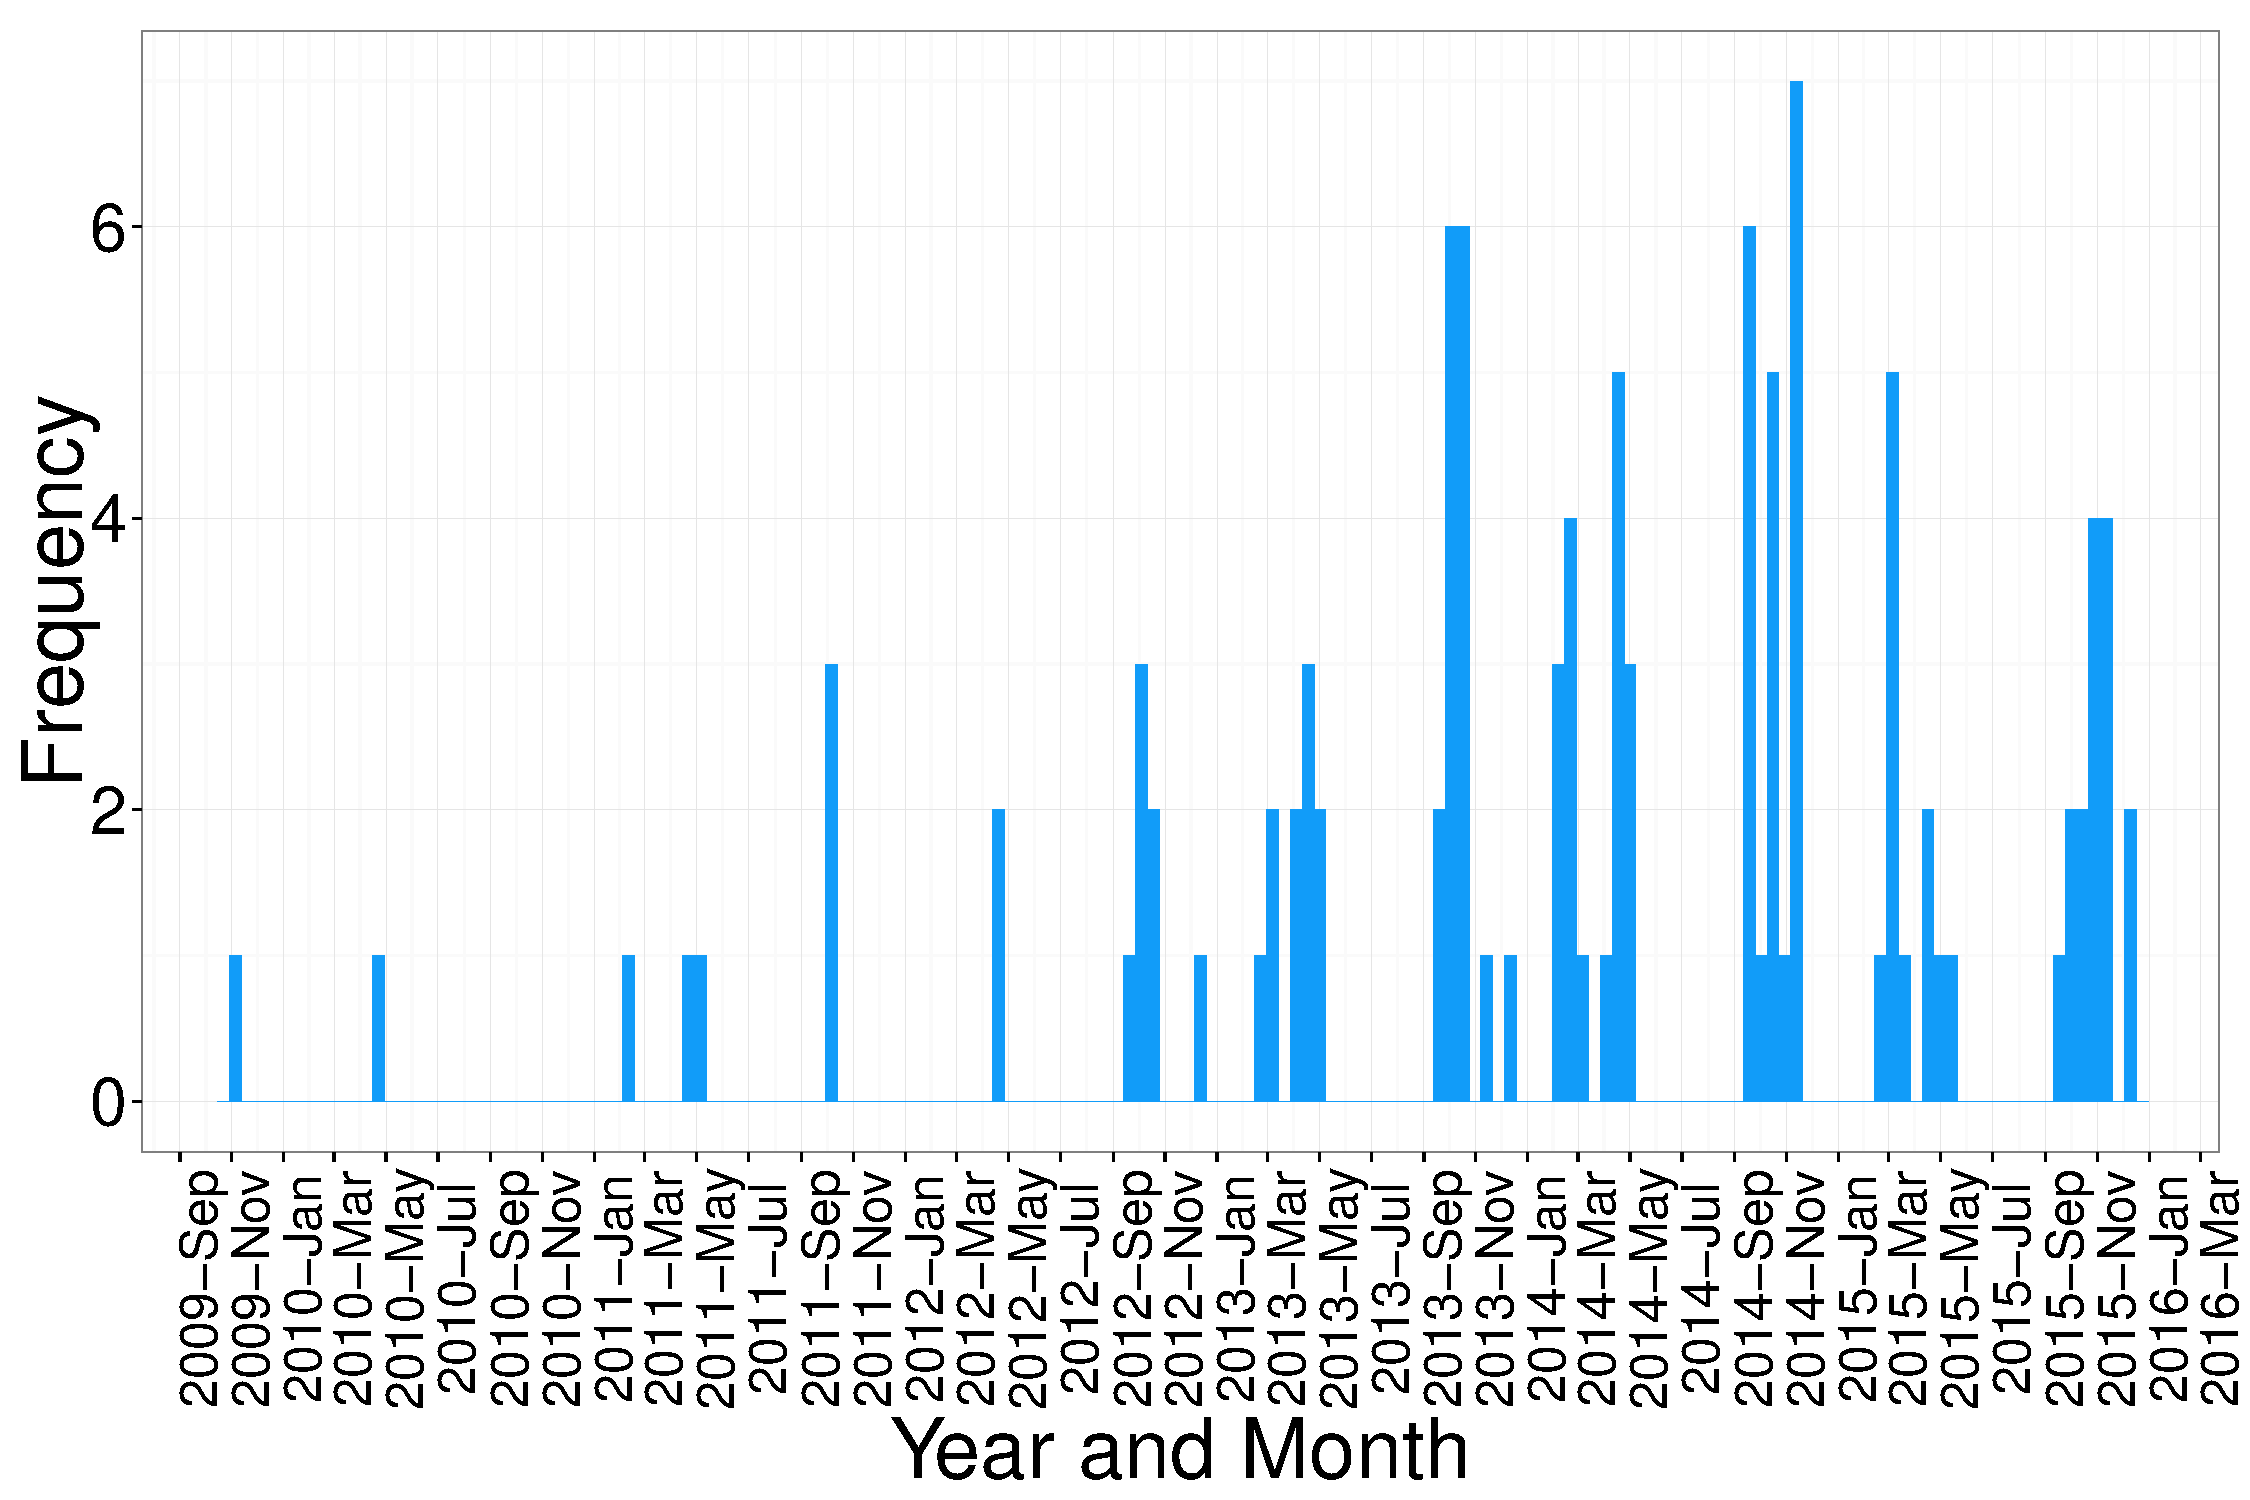
\includegraphics{FinalProject-008}

The trend is quite dramatic: Sexual assault was rarely covered in \textit{TSL} before 2012, but it quickly gained prominence starting in 2013 and appears to have peaked in 2014. This is pretty consistent with national coverage of college sexual assault. The White House published its first report on college sexual assault in April 2014, Columbia University student Emma Sulkowicz began carrying a mattress around campus beginning in September 2014, California became the first state to institute an affirmative consent law in September 2014, and Title IX complaints filed against colleges increased from 11 in the 2009-2010 fiscal year to over 37 in the 2013-2014 fiscal year.

From some of the headlines in the visualization, we can see that the Claremont Colleges have undergone a multitude of changes in response to sexual assault beginning in 2013, including changes in party culture, the creation of task forces dedicated to sexual assault, the implementation of bystander training programs like Teal Dot, and the creation of full-time Title IX coordinator positions.

The final topic trend that we found particularly insightful is that related to movements centered around inequality and student movements. Here's the trend that our model produced:

\begin{Schunk}
\begin{Sinput}
> topicgraph(articles,31,2,14)
\end{Sinput}
\end{Schunk}
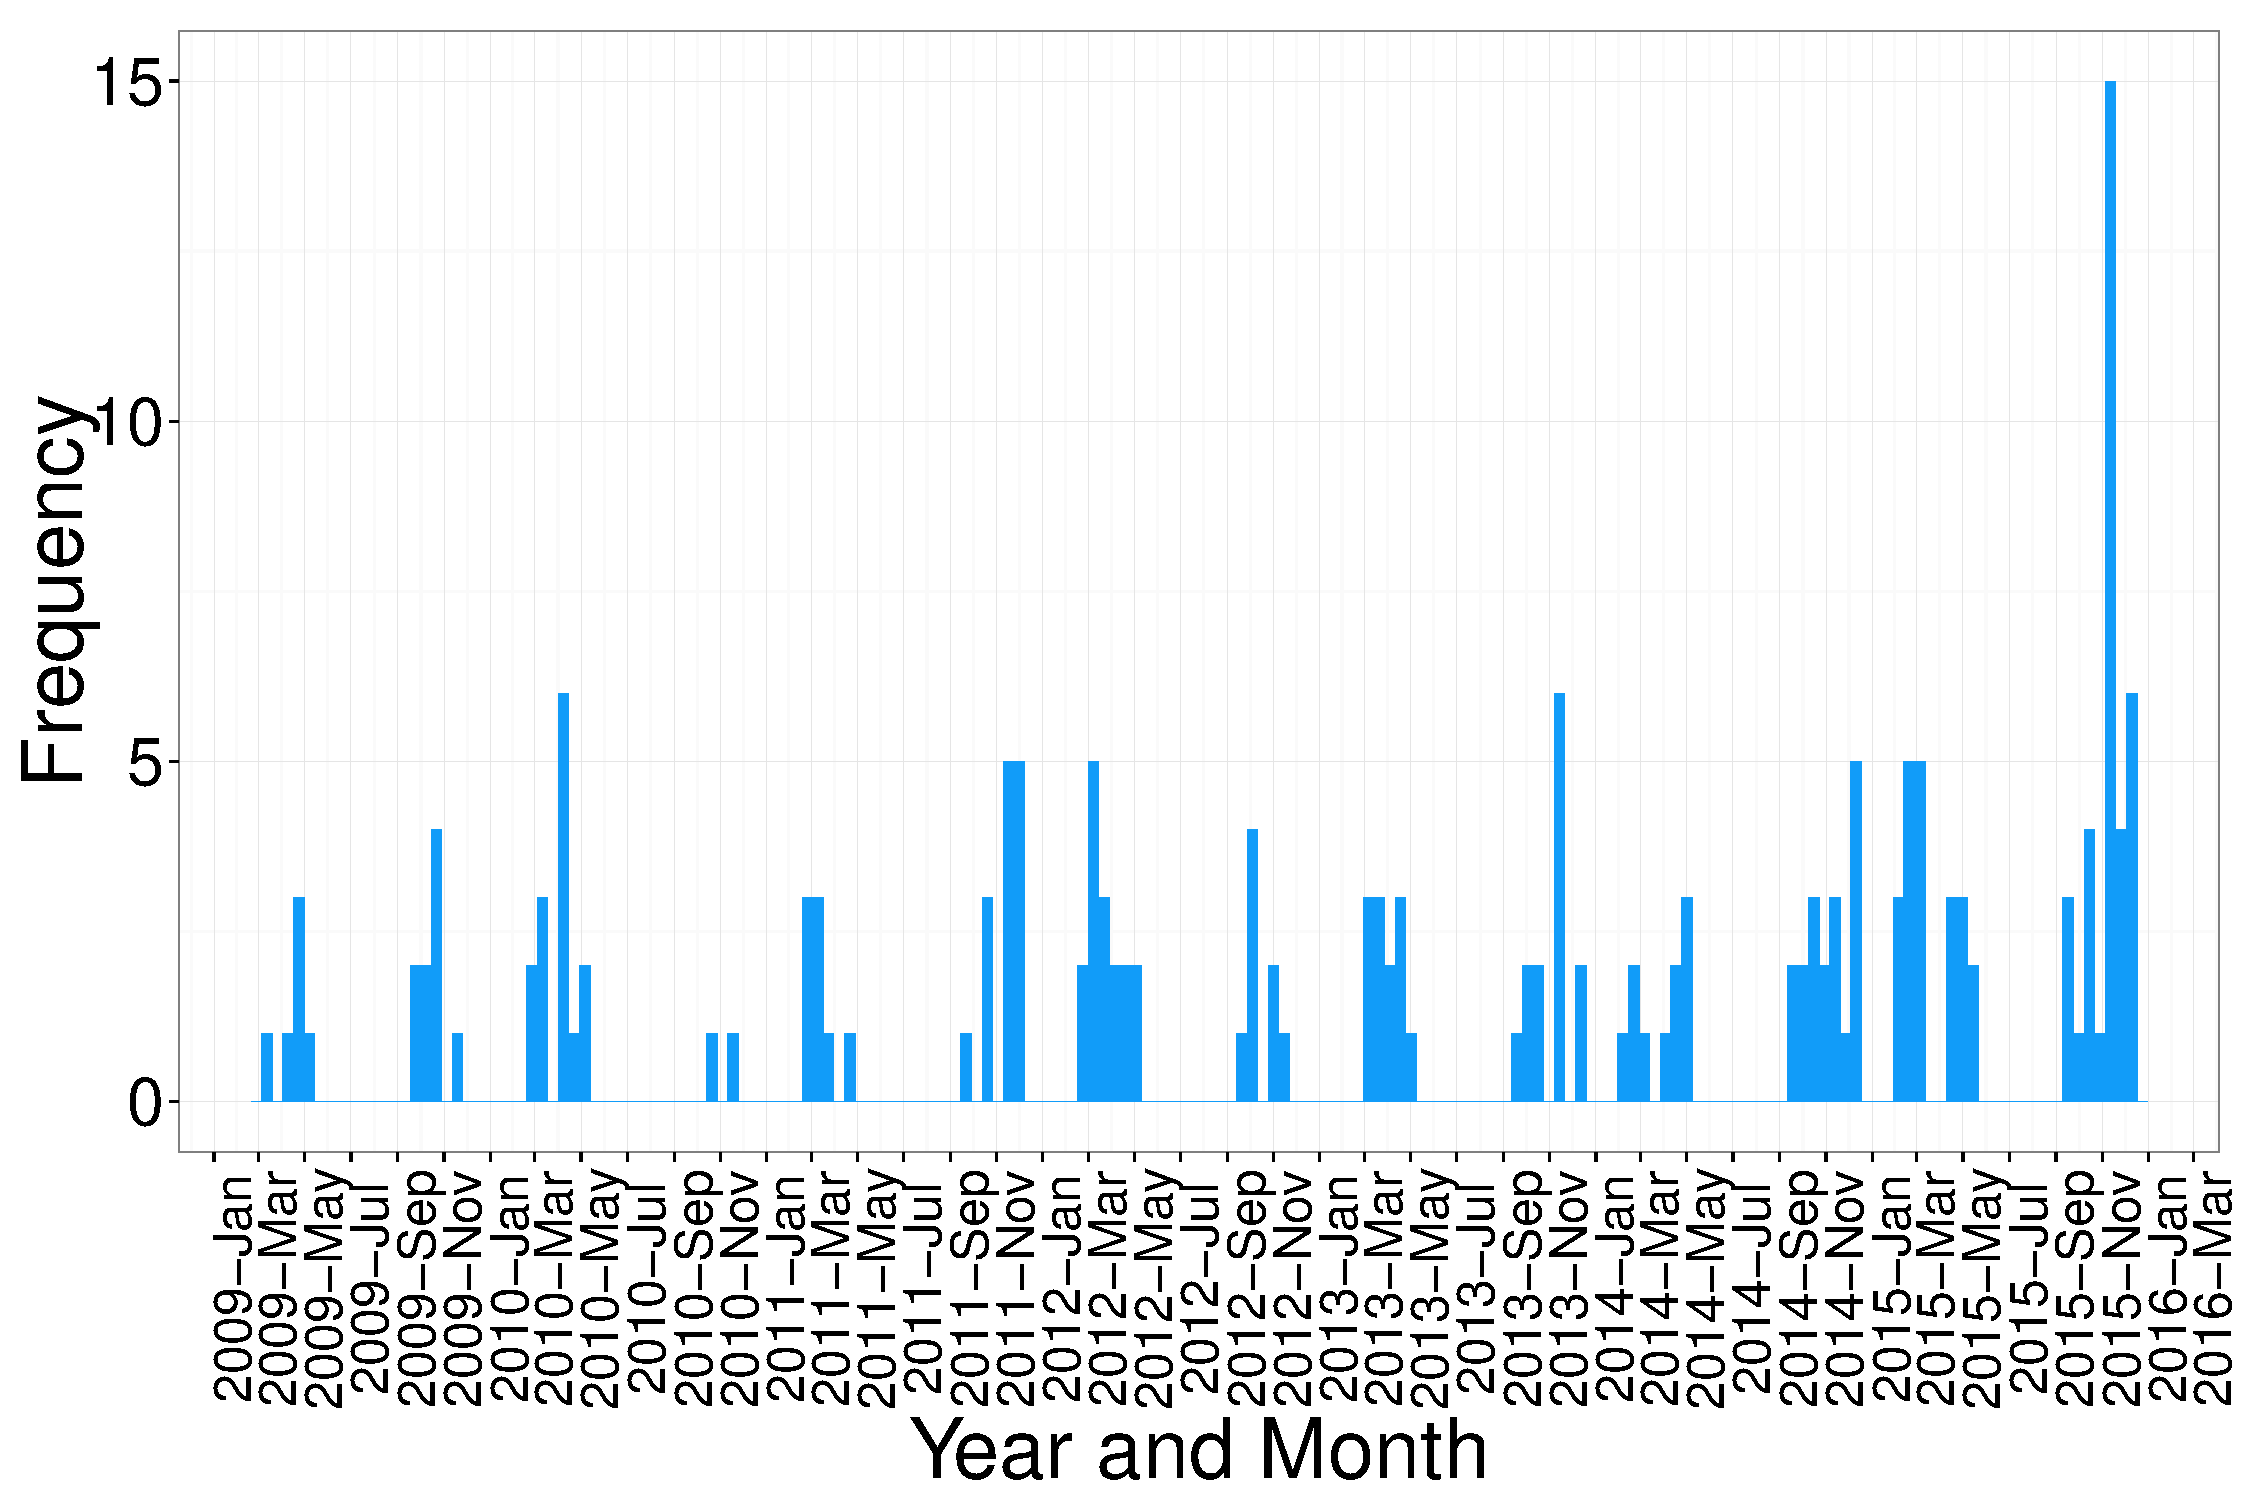
\includegraphics{FinalProject-009}

Based on the graph, it seems that events and discussions centered around inequality (our model appears to overlap racial, sexual, and economic inequality to some degree) have been occurring pretty consistently over time at the Claremont Colleges. We can see that in December 2012, the Occupy Movement gained some coverage by \textit{TSL}. More recently, in December 2014 students reacted to events in Ferguson by marching through the colleges. The most obvious observation, though, is that the topic really blew up in November 2015, when students protested recent events related to race centered at Claremont McKenna College.
[ELABORATE MORE HERE]

Another neat feature of our model is its analysis and visualization of topic coverage by writer. Here's an example:

\begin{Schunk}
\begin{Sinput}
> print(authorChart2(articles,'Diane Lee',2))
> topic.terms[1:10,c(10,19)]
\end{Sinput}
\begin{Soutput}
      Topic 10   Topic 19 
 [1,] "student"  "write"  
 [2,] "discuss"  "book"   
 [3,] "issu"     "read"   
 [4,] "chang"    "stori"  
 [5,] "talk"     "articl" 
 [6,] "question" "tsl"    
 [7,] "campus"   "news"   
 [8,] "import"   "writer" 
 [9,] "pomona"   "media"  
[10,] "colleg"   "publish"
\end{Soutput}
\end{Schunk}
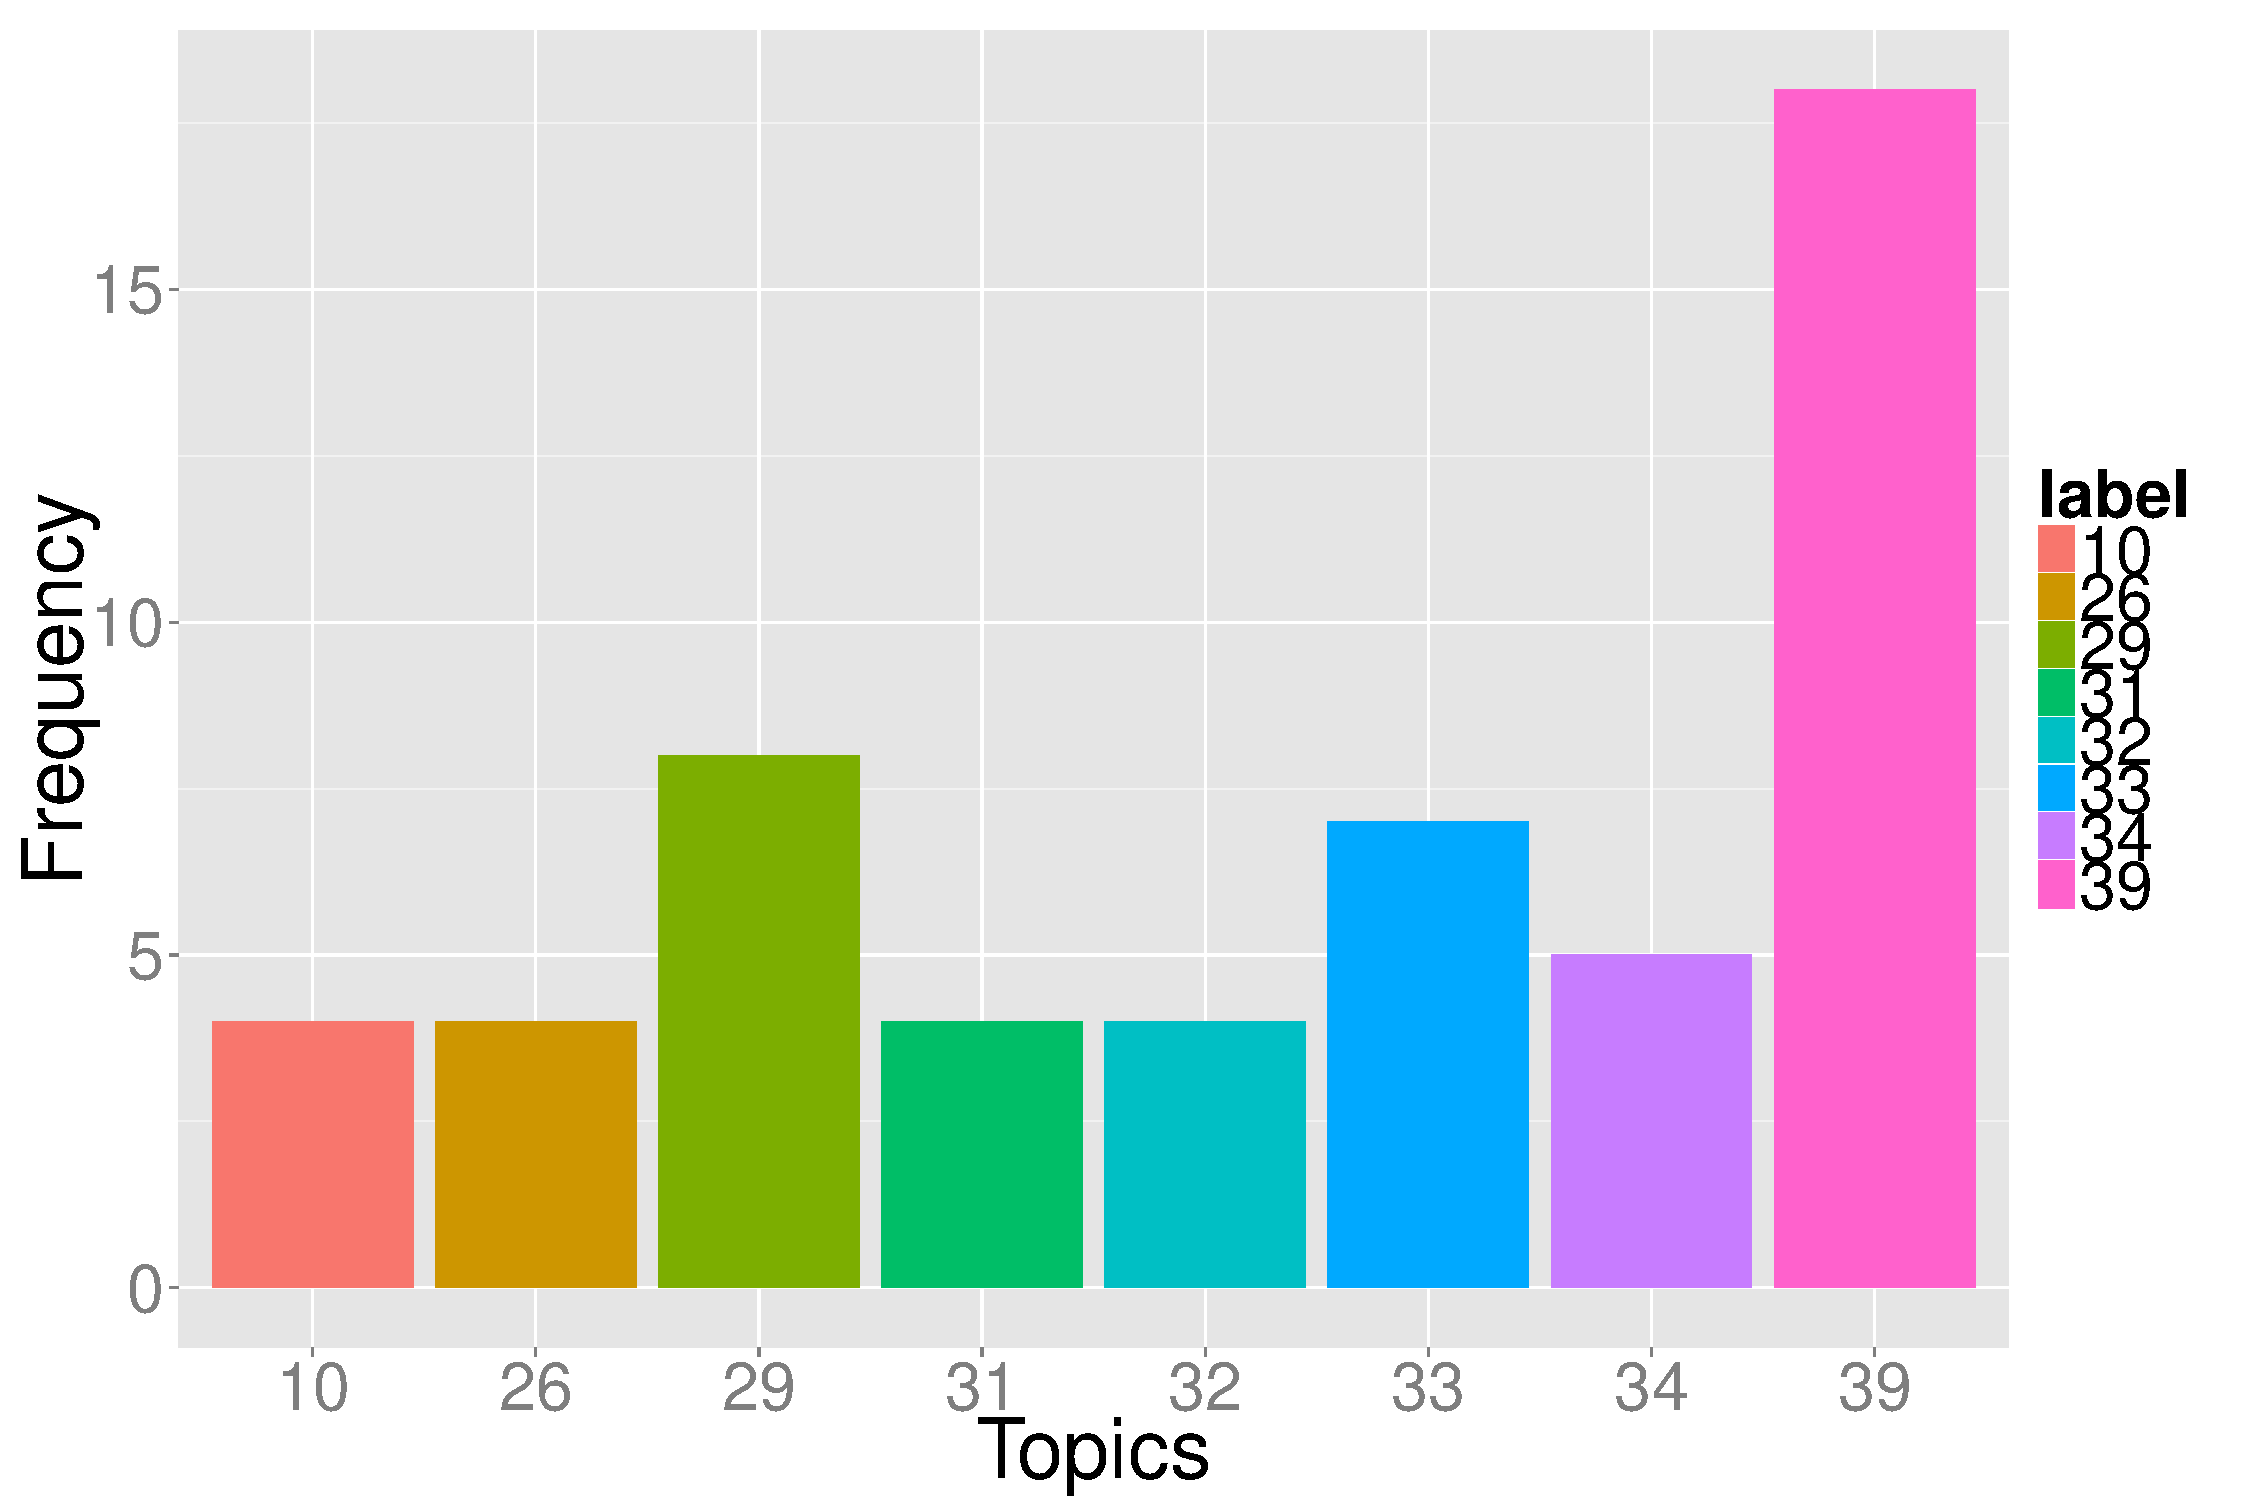
\includegraphics{FinalProject-010}

The graph shows the topics the writer has written the most about. In this case, we can see that Diane Lee wrote a lot of pieces on administrative actions and decisions at the Claremont Colleges.
[maybe elaborate on her positions through the years]

Here's another example:

\begin{Schunk}
\begin{Sinput}
> print(authorChart2(articles,'Sana Kadri',2))
> topic.terms[1:10,c(10,19)]
\end{Sinput}
\begin{Soutput}
      Topic 10   Topic 19 
 [1,] "student"  "write"  
 [2,] "discuss"  "book"   
 [3,] "issu"     "read"   
 [4,] "chang"    "stori"  
 [5,] "talk"     "articl" 
 [6,] "question" "tsl"    
 [7,] "campus"   "news"   
 [8,] "import"   "writer" 
 [9,] "pomona"   "media"  
[10,] "colleg"   "publish"
\end{Soutput}
\end{Schunk}
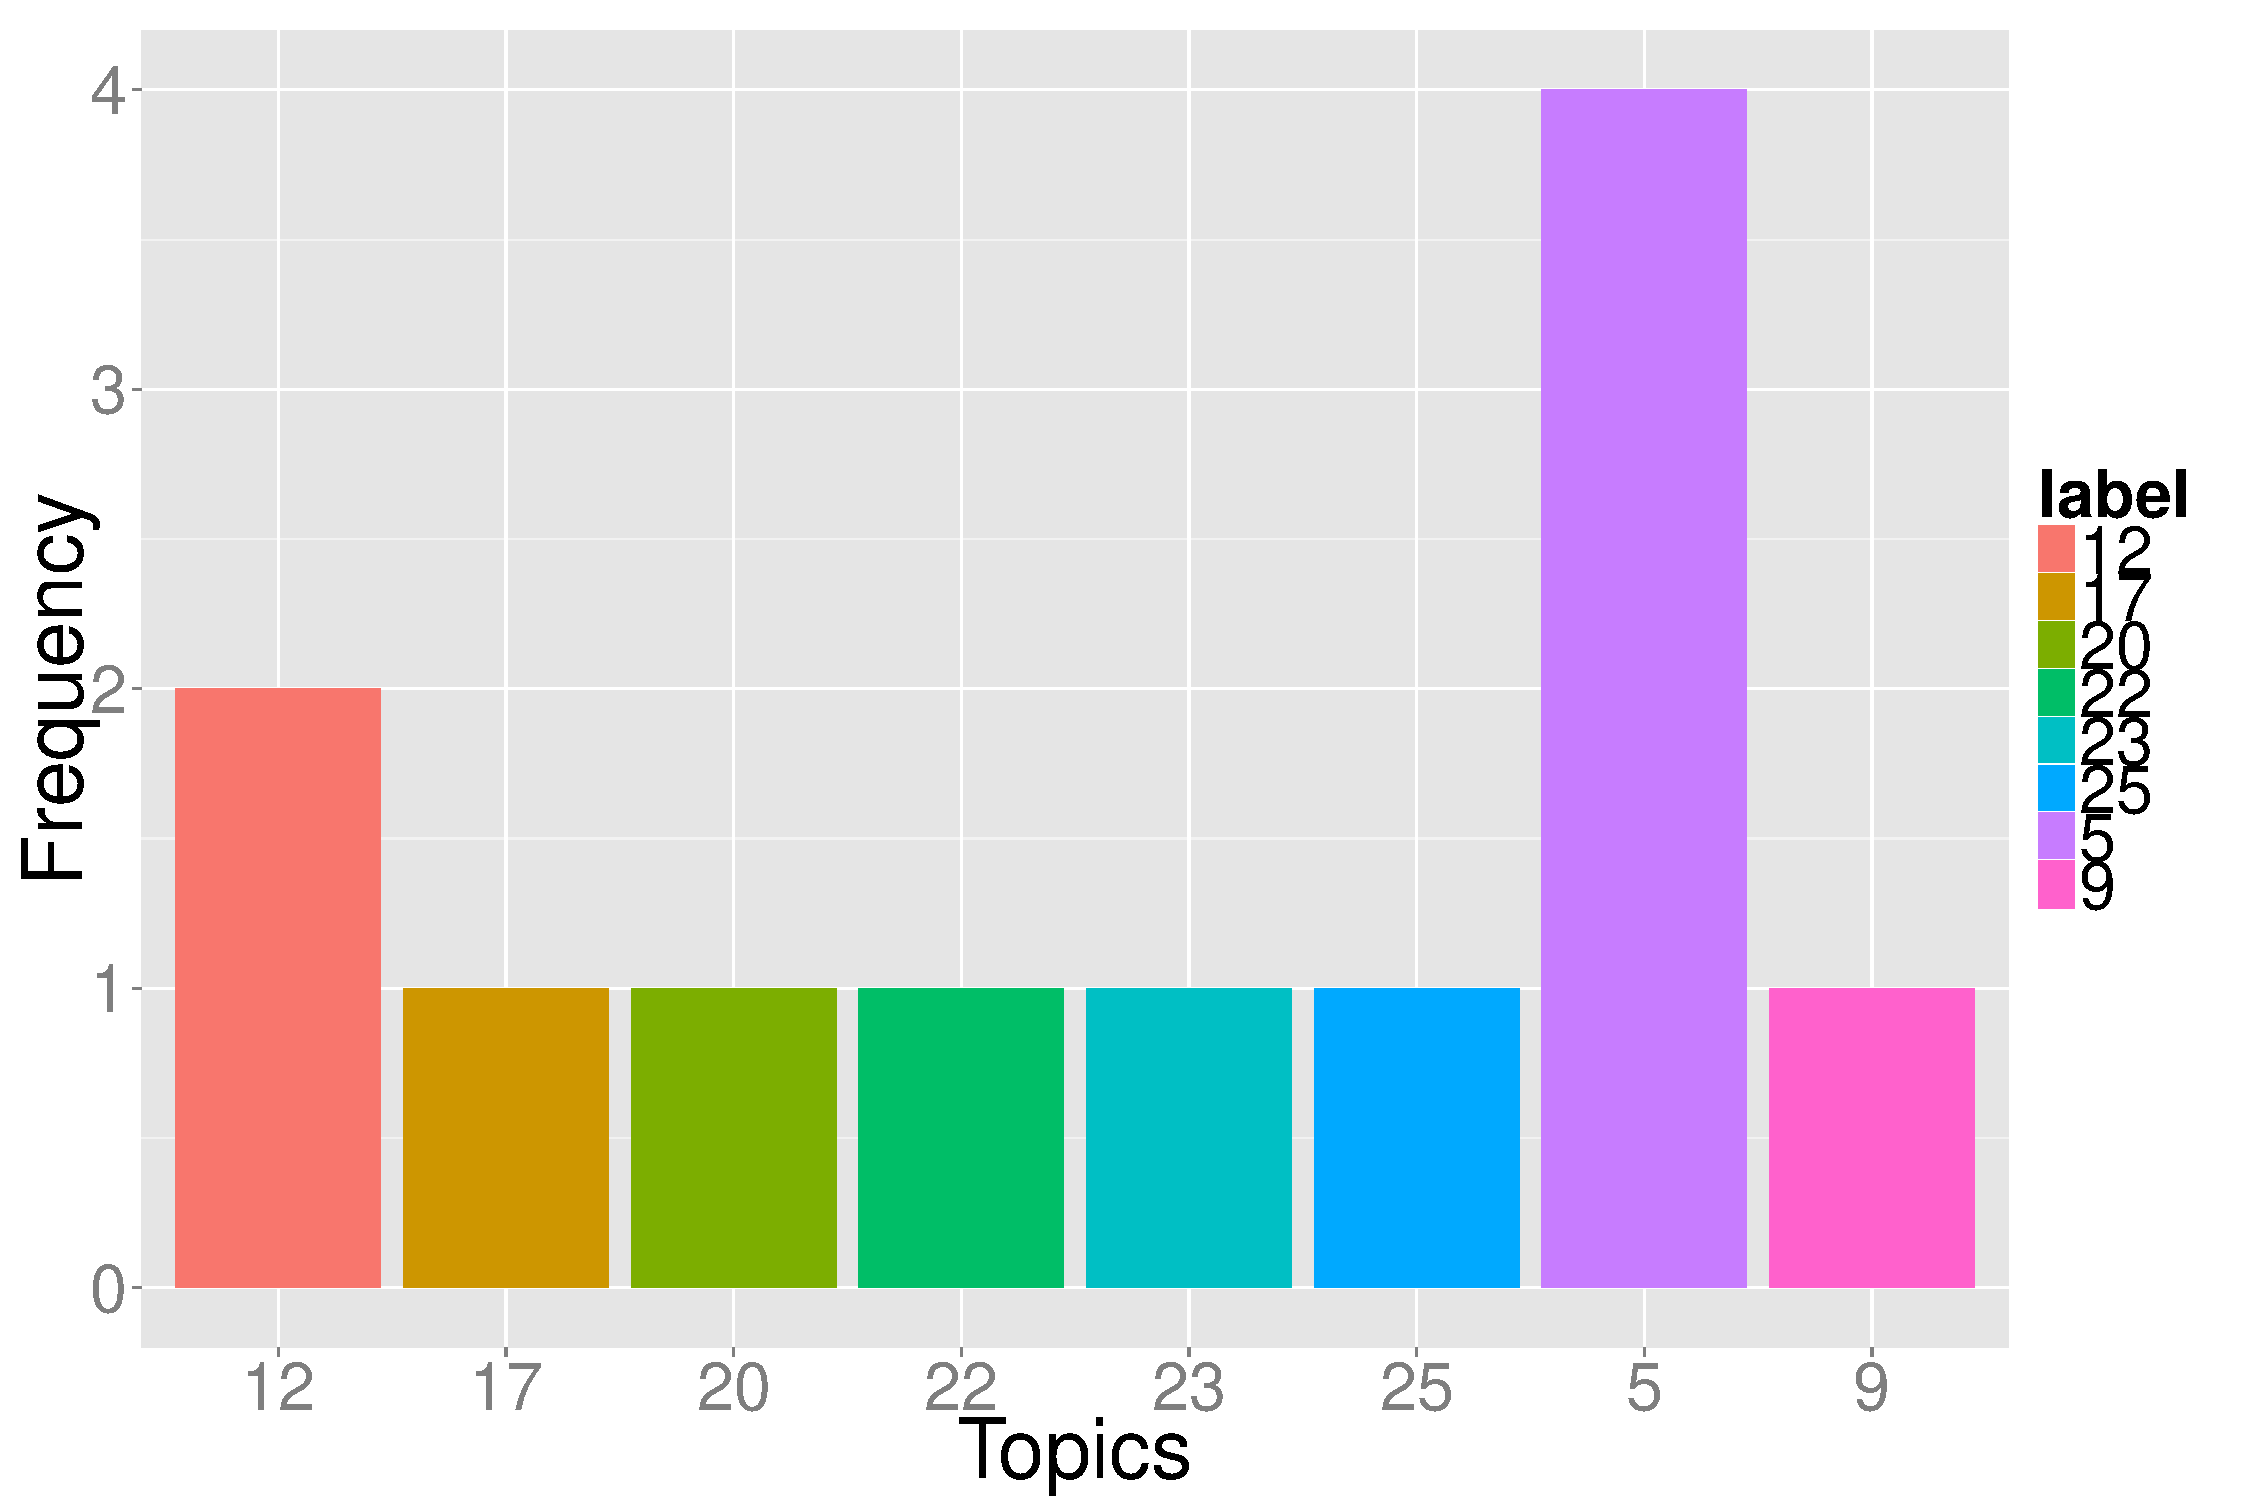
\includegraphics{FinalProject-011}

It seems like Sana Kadri wrote a lot about internationalism and race for \textit{TSL}. Our team for this project includes the opinions editor for \textit{TSL} this semester, who can confirm that Sana, who was an opinions columnist, was very passionate about those topics.

Finally, we can examine the topic content of articles written by the editorial board of \textit{TSL}. Each issue, the editorial board, which consists of the editor-in-chief and the two managing editors, writes a brief editorial that is published in the opinions section. Often, it reflects on another article printed in the same issue. Here's the topic content analysis of the editorial board's pieces:

\begin{Schunk}
\begin{Sinput}
> print(authorChart2(articles,'Editorial Board',2))
> topic.terms[1:10,c(10,19)]
\end{Sinput}
\begin{Soutput}
      Topic 10   Topic 19 
 [1,] "student"  "write"  
 [2,] "discuss"  "book"   
 [3,] "issu"     "read"   
 [4,] "chang"    "stori"  
 [5,] "talk"     "articl" 
 [6,] "question" "tsl"    
 [7,] "campus"   "news"   
 [8,] "import"   "writer" 
 [9,] "pomona"   "media"  
[10,] "colleg"   "publish"
\end{Soutput}
\end{Schunk}
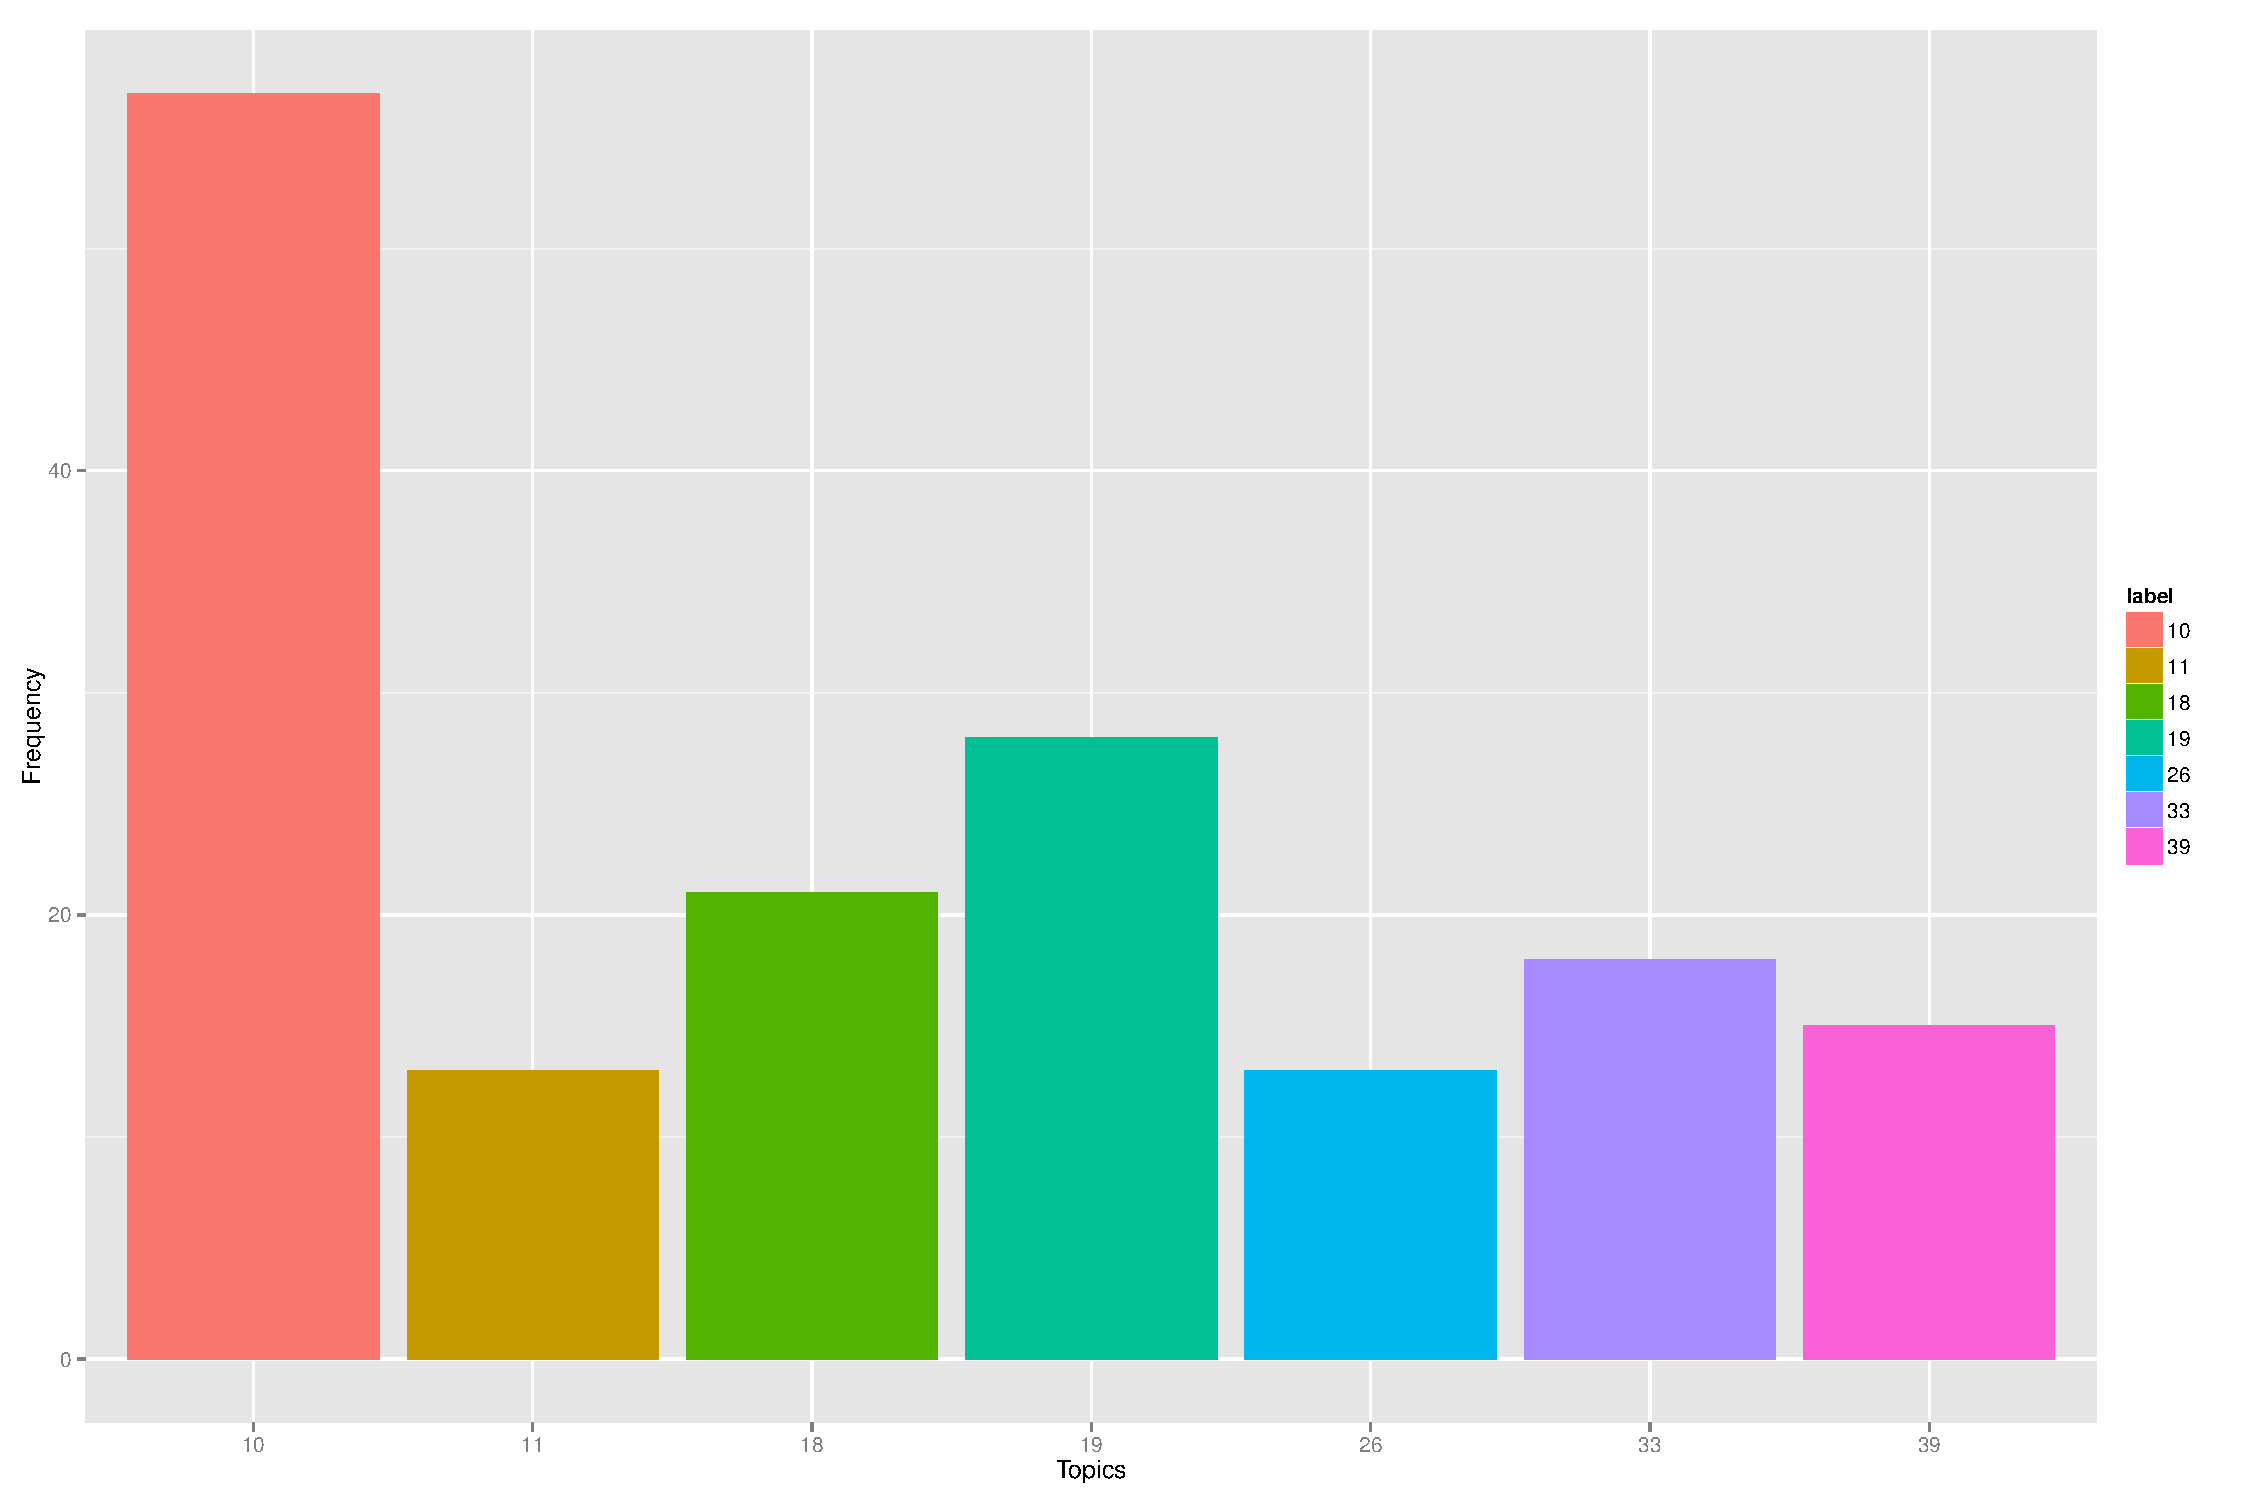
\includegraphics{FinalProject-012}

The chart indicates that the editorial board seems to focus primarily on on-campus issues related to inequality. This would make sense, since events related to such issues often occur and are covered by \textit{TSL}. Also, these issues often generate a lot of discussion and, at times, controversy on campus, making them relevant and appealing topics of conversation for the editorial board to discuss.

\subsection{Miscellaneous Insights}


\subsection{Miscellaneous Insights}


There's a lot to be learned from the data beyond the topic content analysis. For example, with a little bit of wrangling and visualization, we were able to arrive at some interesting findings that might be of some value to the staff at \textit{TSL}. For example, it's no secret that the newspaper struggles with retaining staff writers. But just how bad is it? By tracking the date of each writer's first published article and the writer's last published article, we were able to get a sense of how long they wrote for the paper. Plotting the data, we got the following graph:


\begin{Schunk}
\begin{Sinput}
> retention %>%
+   group_by(semestersTotal) %>%
+   summarise(n = n()) %>%
+   ggplot(aes(x = semestersTotal)) + geom_line(aes(y=n)) + geom_point(aes(y=n)) +
+   xlab('Number of Semesters Writing for TSL') + ylab('Number of Writers') +
+   ggtitle('Retention Rate of TSL Writers') +
+   scale_x_continuous(limits=c(1,13),breaks=seq(0,13,2))
\end{Sinput}
\end{Schunk}
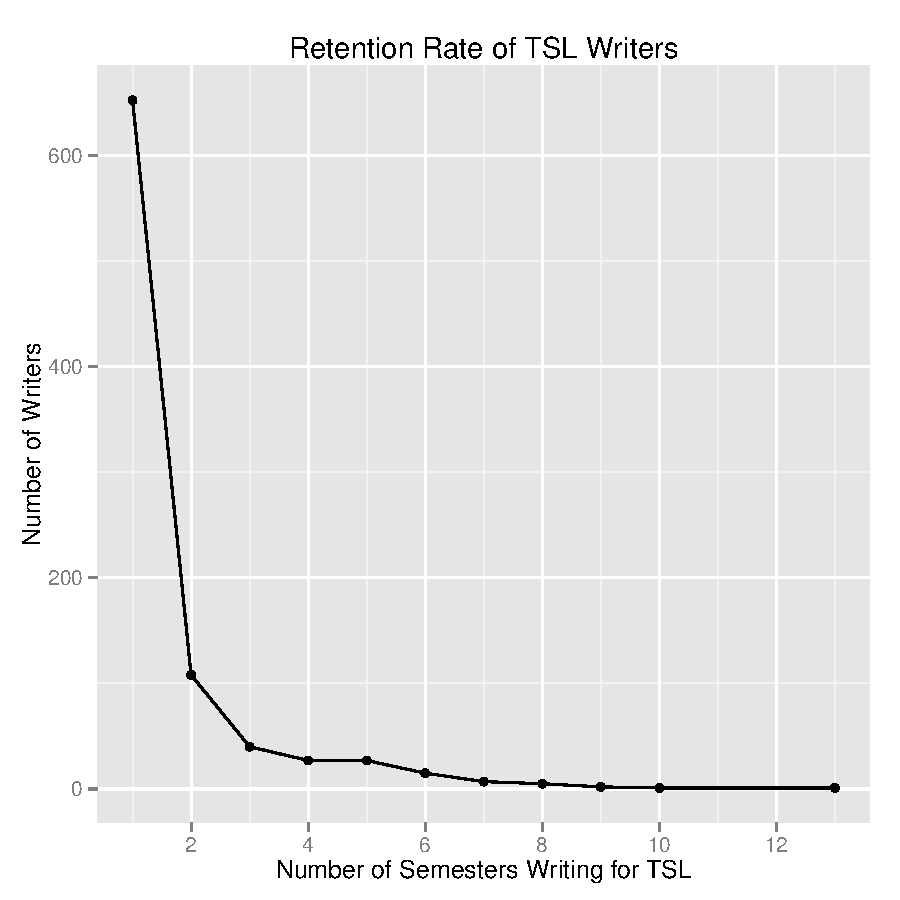
\includegraphics{FinalProject-015}



It seems like \textit{TSL}'s reputation for shedding writers isn't exaggerated. Out of the pool of writers over the past five years, 652 writers stay for one semester or less; 108 writers stay for two semesters; 40 stay for three; and 85 stay for four or more semesters. There are a few caveats, though. First, since the database only includes articles published within the last five years, it's possible that some writers who were seniors when the data first began being collected had been writing for \textit{TSL} for many semesters but are represented as only writing for one semester because their earlier articles aren't included in the database. This might lead to an overestimate of the number of writers who only stay for one or two semesters. Second, the method we applied above to calculate retention reports the difference between the first semester they began writing for \textit{TSL} and the last semester they wrote for \textit{TSL}. Some writers, however, take a semester or more off from writing for \textit{TSL} to study abroad or simply pursue other interests before returning to write again. In these cases, the number of semesters they spent writing for \textit{TSL} are overestimated. These cases probably consistute only a small minority of the data points, however, so the overall trend still holds.

We can easily track the retention rate by section as well:

\begin{Schunk}
\begin{Sinput}
> retention %>%
+   filter(section_id != 5) %>%
+   group_by(semestersTotal, section_id) %>%
+   summarise(n = n()) %>%
+   ggplot(aes(x = semestersTotal, y=n, color=factor(section_id))) + geom_point() +
+   geom_line() + scale_color_discrete(name="Section", labels =
+   c('News','Sports','Opinions','L&S')) + xlab('Number of Semesters Writing for TSL') +
+   ylab('Number of Writers') + ggtitle('Retention Rate by Section') +
+   scale_x_continuous(limits=c(1,13),breaks=seq(0,13,2))
\end{Sinput}
\end{Schunk}
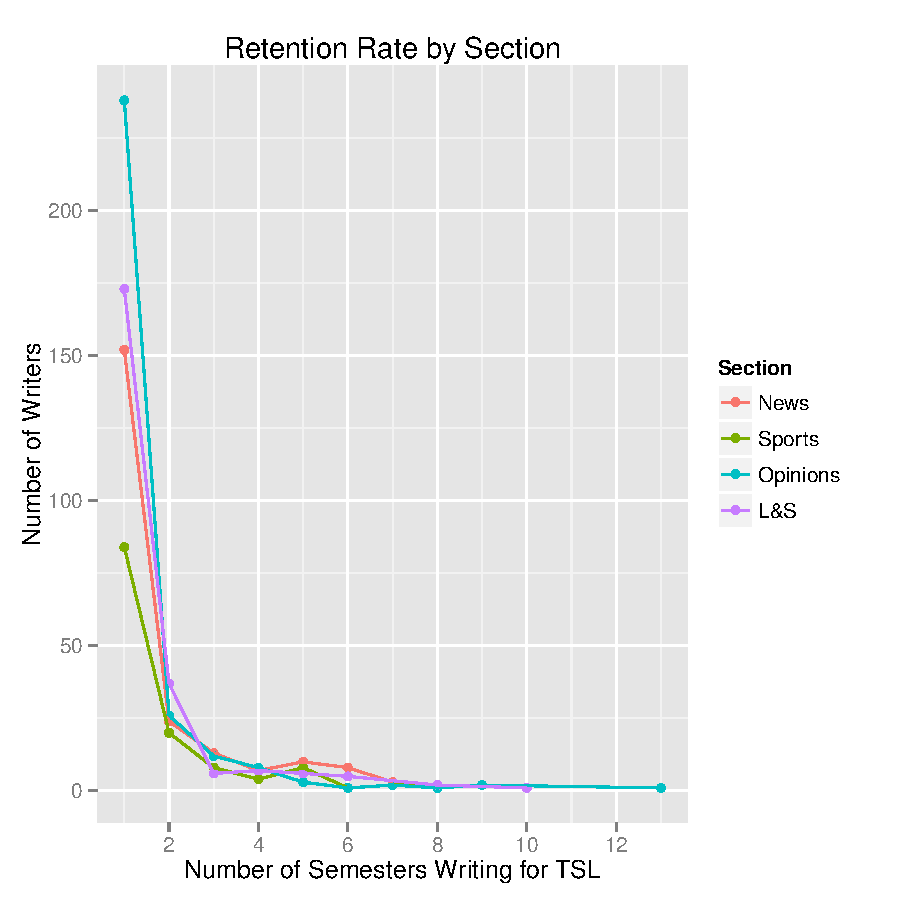
\includegraphics{FinalProject-016}

It seems like the opinions section suffers the steepest drop in returning writers. A lot of this may be attributable to the fact that anywhere from one-fourth to one-half of the articles in the opinions section each week are written by guest writers, who typically write only for a single, specific event or issue. Unfortunately, we can't filter those writers out given the data that we have.

Another area of interest might be how prolific writers for \textit{TSL} are--that is, how many articles each writer writes. It seems pretty reasonable to expect that trend to resemble the retention rates shown above. After all, a person can only write so many articles if they're only a writer for one semester. And indeed, we can see that this is the case:


\begin{Schunk}
\begin{Sinput}
> articles_per_writer %>%
+   ggplot(aes(x = total)) + geom_histogram(binwidth = 1, col=I('gray')) +
+   ggtitle('Histogram of Articles per Writer') +
+   xlab('Number of Articles Written') + ylab('Number of Writers')
\end{Sinput}
\end{Schunk}


We can also break it down by section:

\begin{Schunk}
\begin{Sinput}
> sections = c('News','LS','Opinions','Sports')
> for (num in 1:4) {
+   section <- sections[num]
+   assign(paste(section, 'section_articles_per_writer', sep='_'), articles %>%
+     filter(section_id == num) %>%
+     group_by(profile_id) %>%
+     summarise(total = n()) %>%
+     ggplot(aes(x = total)) + geom_histogram(binwidth = 1, col=I('gray')) +
+     ggtitle(section) + xlab('Number of Articles Written') + ylab('Number of Writers'))
+ }
> grid.arrange(News_section_articles_per_writer,Opinions_section_articles_per_writer,
+              LS_section_articles_per_writer,Sports_section_articles_per_writer, ncol=2)
\end{Sinput}
\end{Schunk}
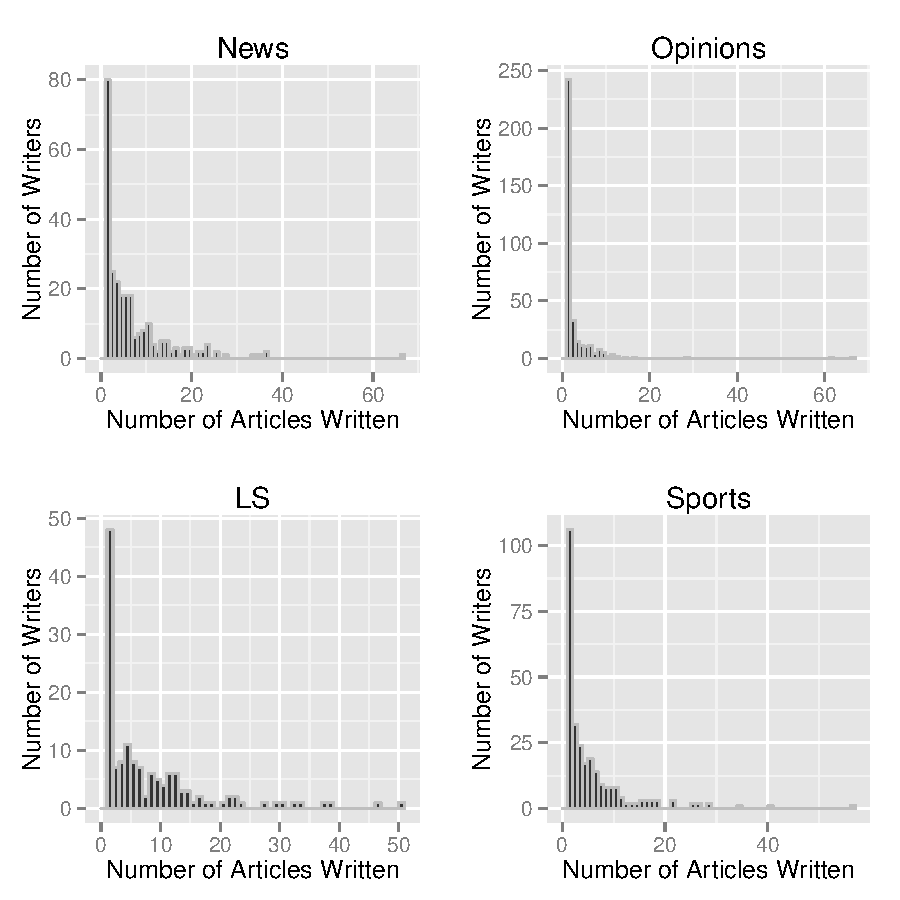
\includegraphics{FinalProject-019}



Finally, we were able to get a sense of how popular articles published this semester have been by looking at the number of times each article was visited. Because data on the number of visitors to each article only began being collected in the fall semester of 2015, we had to limit our analysis to articles in that time period. Below are the top 10 most-viewed articles from the fall:

\begin{Schunk}
\begin{Soutput}
                                                                                          title
1                                     Who Is the Happiest at the "Happiest College in America"?
2                     This Year's Pomona Essay Questions Discourage Underrepresented Applicants
3  CMC Students of Color Protest for Institutional Support, Call for Dean of Students to Resign
4                                CMC’s Black Students See Low Graduation Rates, Lack of Support
5                                          Amid Calls for Resignation, Dean Spellman Steps Down
6                                                                   Why I Left (Pomona College)
7                                                    Pomona College Receives Title IX Complaint
8                                                     Break the Mold: Why I Won’t Donate to CMC
9                                           Pomona Taco Crawl: The Must-See Taquerias in Pomona
10                               Even in Foam and Plastic, Gun  Violence Does Not Belong at 5Cs
   published_date             author_name clicks
1      2015-10-23        Lisette Espinosa  22012
2      2015-11-06            Chuck Herman   8602
3      2015-11-11          Kevin Tidmarsh   8251
4      2015-10-09          Sam McLaughlin   4162
5      2015-11-12          Kevin Tidmarsh   3862
6      2015-11-06 Conner Bouchard-Roberts   3669
7      2015-10-09          Kevin Tidmarsh   3577
8      2015-11-11       Aseem Chipalkatti   2467
9      2015-09-18        Joaquin Banuelos   2187
10     2015-10-09          Benjamin Cohen   2129
\end{Soutput}
\end{Schunk}


For those who are familiar with recent events on campus this semester, the list makes sense. For example, Lisette Espinosa emailed her opinions piece to Claremont McKenna College's former Dean of Student Mary Spellman, who gave a controversial reply that, some would argue, led to her resignation. Indeed, it seems like a lot of the top articles are related to issues of race, sexual assault, campus climate, and college image. 

Similarly, we can identify the most-viewed writers on average:

\begin{Schunk}
\begin{Soutput}
Source: local data frame [10 x 3]

               author_name average_views articles_published
                    (fctr)         (dbl)              (int)
1         Lisette Espinosa     22012.000                  1
2             Chuck Herman      8602.000                  1
3  Conner Bouchard-Roberts      3669.000                  1
4           Kevin Tidmarsh      2637.714                  7
5        Aseem Chipalkatti      2467.000                  1
6           Benjamin Cohen      2129.000                  1
7            Adin Bonapart      1648.000                  1
8         Joaquin Banuelos      1270.500                  2
9         Carol Ann  Routh      1174.000                  1
10            Tom Schumann      1167.000                  1
\end{Soutput}
\end{Schunk}

A lot of these are one-hit writers, which makes sense. The opinions section regularly invites guest writers to publish a piece in the paper. Typically, when this happens, the guest writer writes about a particularly controversial or timely subject; that is what motivates them to write, after all. As such, their pieces often get a lot of views. On the other hand, the other sections' pieces are written by regular staff writers, who have to cover the mundane along with the occasional big events each semester. Since the guest writers typically only write once about a hot-button issue, it makes sense that many of the most-viewed writers have only written once for the newspaper.

Nonetheless, we might be interested in seeing which regular contributors to the paper's content get the most views:

\begin{Schunk}
\begin{Soutput}
Source: local data frame [10 x 3]

          author_name average_views articles_published
               (fctr)         (dbl)              (int)
1      Kevin Tidmarsh     2637.7143                  7
2      Sam McLaughlin     1104.1667                  6
3          Sana Kadri      608.7500                  4
4     Editorial Board      603.7000                 10
5  William Schumacher      587.2500                  4
6       Elizabeth Lee      471.8333                  6
7          Sean Ogami      442.5556                  9
8      Harini Salgado      432.0000                  5
9           Diane Lee      429.8000                  5
10       Natalie Quek      396.5000                  4
\end{Soutput}
\end{Schunk}

We now move from examining individual view counts to examining the aggregate data. Here's a boxplot of article views for articles published in fall 2015:

\begin{Schunk}
\begin{Sinput}
> # plot distribution of views in fall 2015
> clicks %>%
+   ggplot(aes(x = semester, y = clicks)) + geom_boxplot() + xlab('Semester') +
+   ylab('Cumulative Number of Clicks') +
+   ggtitle('Distribution of Clicks of TSL Fall 2015 Articles')
\end{Sinput}
\end{Schunk}
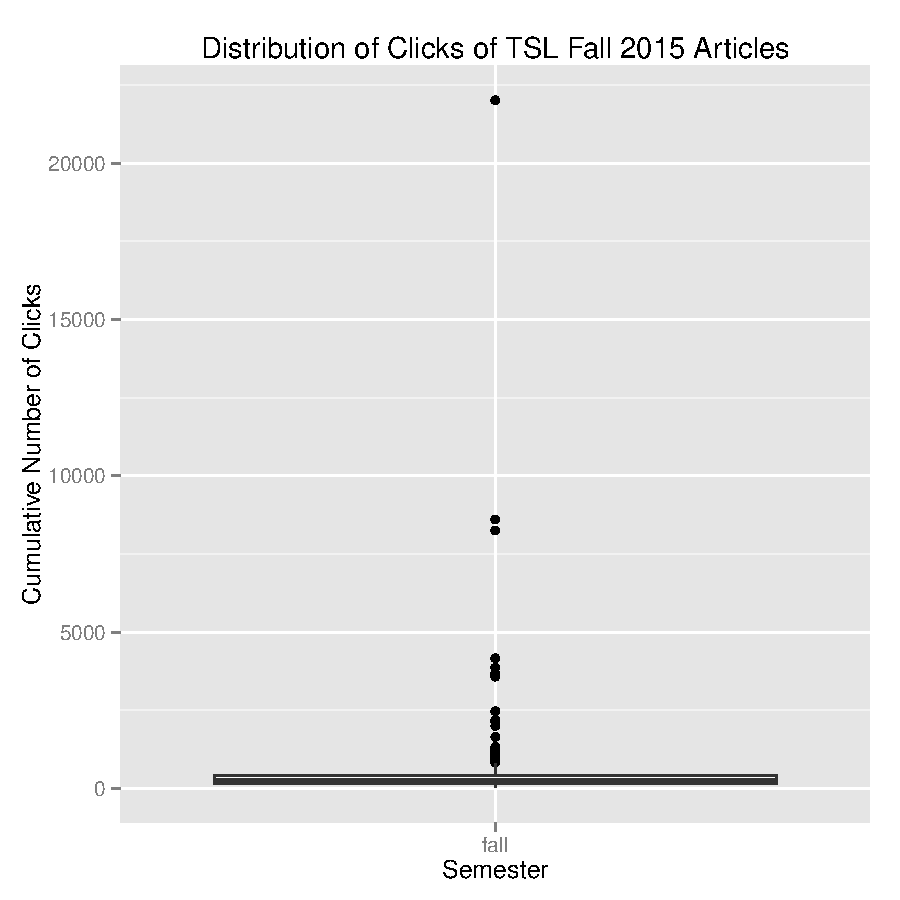
\includegraphics{FinalProject-024}


We can see that there are some extreme outliers---the articles from the most-viewed list above---that make it difficult to look at the rest of the observations, so we'll focus our view on the bulk of the data:

\begin{Schunk}
\begin{Sinput}
> # exclude outliers from view
> clicks %>%
+   ggplot(aes(x = semester, y = clicks)) + geom_boxplot() +
+   scale_y_continuous(limits = c(0,500)) + xlab('Semester') +
+   ylab('Cumulative Number of Clicks') +
+   ggtitle('Distribution of Clicks of TSL Fall 2015 Articles')
\end{Sinput}
\end{Schunk}
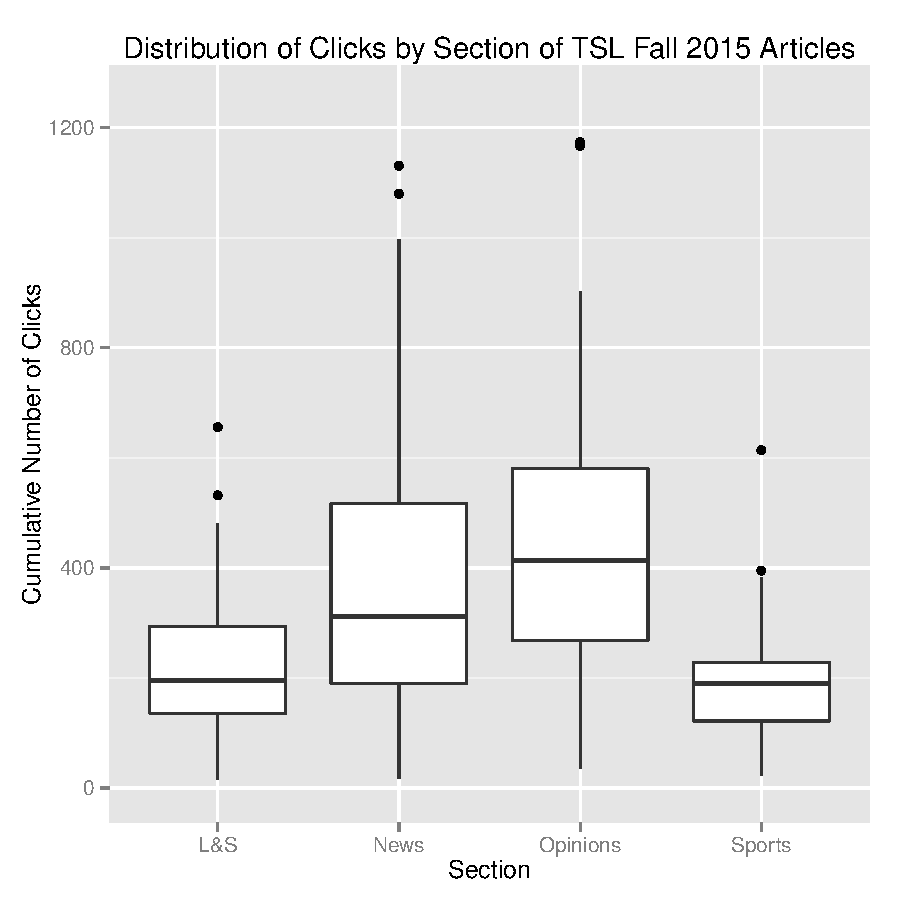
\includegraphics{FinalProject-025}


The median article published this semester, arranged by number of views, was viewed just over 200 times. The upper quartile of articles are viewed at least 300 times each, while the lower quartile are viewed at most about 145 times each.

We can break the data down by section too:

\begin{Schunk}
\begin{Sinput}
> # do the same as above but by section
> clicks %>%
+   filter(section_id != 5) %>%
+   mutate(section = ifelse(section_id==1, 'News', ifelse(section_id==2, 'Sports',
+   ifelse(section_id==3, 'Opinions', 'L&S')))) %>%
+   ggplot(aes(x = factor(section), y = clicks)) + geom_boxplot() +
+   xlab('Section') + ylab('Cumulative Number of Clicks') +
+   ggtitle('Distribution of Clicks by Section of TSL Fall 2015 Articles')
\end{Sinput}
\end{Schunk}
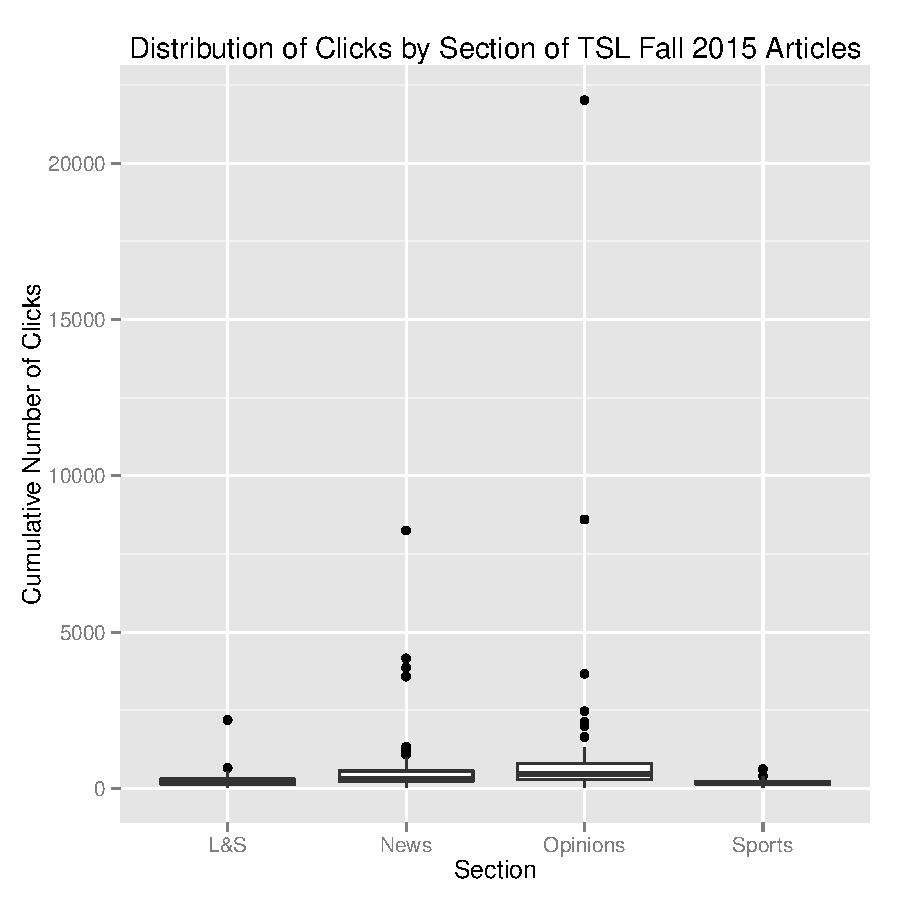
\includegraphics{FinalProject-026}

Focusing on the bulk of the observations: 

\begin{Schunk}
\begin{Sinput}
> # exclude outliers from view
> clicks %>%
+   filter(section_id != 5) %>%
+   mutate(section = ifelse(section_id==1, 'News', ifelse(section_id==2, 'Sports',
+   ifelse(section_id==3, 'Opinions', 'L&S')))) %>%
+   ggplot(aes(x = factor(section), y = clicks)) + geom_boxplot() +
+   scale_y_continuous(limits = c(0,1250)) + xlab('Section') +
+   ylab('Cumulative Number of Clicks') +
+   ggtitle('Distribution of Clicks by Section of TSL Fall 2015 Articles')
\end{Sinput}
\end{Schunk}
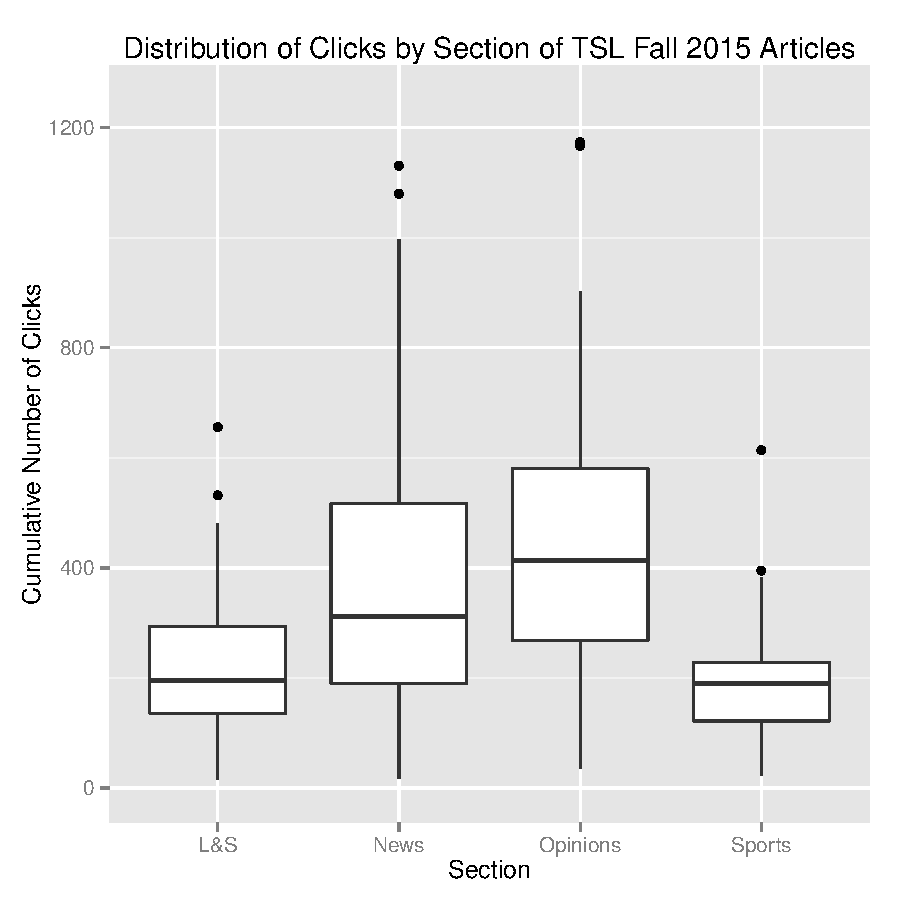
\includegraphics{FinalProject-027}

It seems like opinions pieces are viewed the most, though news pieces are not far behind. Articles in the sports and life \& style section, though, are not viewed as much; the upper quartile for sports articles is below the lower quartile for opinions pieces, and the upper quartile for life \& style articles is not much higher. This makes sense given the atmosphere at the Claremont Colleges. Students generally seem less interested in topics covered in sports and life and style pieces than they are in topics covered in news and opinions pieces.




















\section{End Product}
This project is not only about gaining insights into student discourse, but also about creating an infrastructural tool that allows other interested students to find answers to their own questions about our history. With that goal in mind, we created an interactive shiny app that can respond to users' queries on different topics, authors and articles and then generate plots or perform analyses similar to those in this report. The app is online at \href{https://ziqixiong.shinyapps.io/TopicAnalysis}{https://ziqixiong.shinyapps.io/TopicAnalysis}.
\vspace{1cm}

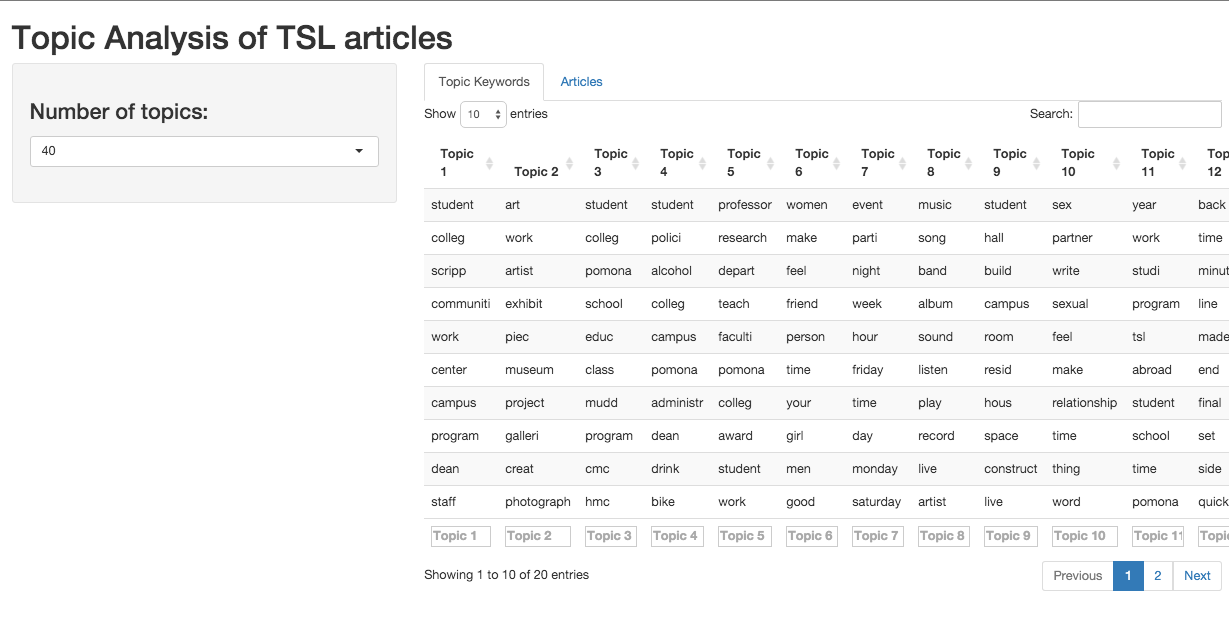
\includegraphics[width=300px]{shinydemo.png}

\section{Conclusion}
\subsection{Summary}
After building models through Latent Dirichlet Allocation of the corpus of \textit{TSL} articles over the past five years, we were able to track how much coverage various subjects received in \textit{TSL} over time. From this, a rough idea of how these topics have been trending over time can be ascertained. For example, from our model we infer that [insert example]. Using the topic information in conjunction with the articles, authors, and time, many other insights can be gleaned. These include the topic breakdowns for each author and article; that is, how much each author or article falls into certain topics. The models can also be applied in order to analyze the topic breakdowns of new articles, or even entirely different documents. Through this, we aim to provide a tool for more future analysis of TSL discourse, and thus student discourse over time.

\subsection{Limitations}
Our model faces several limitations, regarding both its analysis of topic coverage in \textit{TSL} and the inferences that can reasonably be drawn from its findings. Some of the topics generated through the model creation process are not very useful. For example, there are a few scattered `` Miscellaneous''  topics that have no logical continuity between the articles. The key words used for these miscellaneous topics have little relation to each other. This is bound to happen sometimes, as LDA is an unsupervised method, so we should not necessarily expect it to always find groups that make sense to us. For some numbers of topics, a topic based around weird punctuation or symbols that a few authors use is generated, since these are counted as distinctive words. Sometimes, topics are also combined, as is the case with `` Campus Activism''  combining both the divestment action and the action around the campus worker rights in 2012. On the whole, LDA produced topics that were sensible and comprehensible, ranging from ``Running'' to ``Fashion.'' In the 40 Topic model, for instance, there was only one ``Miscellaneous'' topic and one ``NA'' topic (which was due to the weird symbols used by a few authors). This means that 38/40 topics were useful, which is a very good proportion for an unsupervised method. As with all tools, it is useful so long as the shortcomings are kept in mind.

\subsection{Future Work}
The model could also be improved to enable users to obtain a more accurate understanding of how the prominence of topics in campus discourse has changed over time. Perhaps most obviously, the frequency with which a \textit{TSL} article is visited online over a certain period of time likely is significant indicator of the prominence of the article's main topic during that period of time. Currently, the model does not include such information because the number of visitors was not tracked until this semester. As a result, certain topics are represented by the model as more prominent in campus discourse than perhaps they truly were. For example, our model produces three or four topics that are all essentially athletics. Moreover, since the sports section consistently covers sports events at the Claremont Colleges every issue of the newspaper, the model's visualization shows a consistently moderate number of \textit{TSL} articles covering sports, giving the impression that sports figure relatively prominently in the collective campus conscious. Without prior knowledge of our campus culture, it might be easy for someone to draw such an inference, when in fact athletics has a relatively modest place in campus dialogue. The frequency of visitors to each article would provide a different perspective: As shown in Section 4.2, sports articles generally had fewer online visitors than news and opinions articles this semester, and certain pieces related to race-based issues and Pomona branding received the most visitors. These data points are likely more consistent with the nature of campus discourse this past semester. If the model accounted for this type of information in its visualizations, it would present a more accurate picture of how topics trend over time. The issue of topics that aren't useful to humans can be helped through the implementation of interactivity into the LDA building. Since LDA iterates until reaching a local optima, it can be nudged out of this optima by taking user input, such as ``this word cannot be in this topic.'' This would be more of a power user feature than one for the average user, as it requires computational time to reiterate for topic building. Finally, if it would be possible to obtain and convert data on articles before 2009 into a usable format, this could obviously grant more ability to perform historical analysis.
\end{document}
